\input templates/header

\usepackage{blkarray, bigstrut}
\usepackage{listings}
\lstset{
  basicstyle=\ttfamily,
  columns=fullflexible,
  keywordstyle=\color{red}\bfseries,
  commentstyle=\color{blue},
  showstringspaces=false,
  escapeinside={(*@}{@*)},
}

\newcommand\topstrut[1][1.2ex]{\setlength\bigstrutjot{#1}{\bigstrut[t]}}
\newcommand\botstrut[1][0.9ex]{\setlength\bigstrutjot{#1}{\bigstrut[b]}}


\renewcommand{\mmark}{\mathit{visited}}
\renewcommand{\hascycle}{\mathit{hasCycle}}

\title[ASD - Grafi]{\textbf{Algoritmi e Strutture Dati}\\[24pt]
Grafi}

\graphicspath{{figs/09/}}

\begin{document}



%-------------------------------------------------------------------------
\FrameTitle{}

%-------------------------------------------------------------------------
\FrameContent

%%%%%%%%%%%%%%%%%%%%%%%%%%%%%%%%%%%%%%%%%%%%%%%%%%%%%%%%%%%%%%%%%%%%%%%%%%
\section{Introduzione}
%%%%%%%%%%%%%%%%%%%%%%%%%%%%%%%%%%%%%%%%%%%%%%%%%%%%%%%%%%%%%%%%%%%%%%%%%%

%%%%%%%%%%%%%%%%%%%%%%%%%%%%%%%%%%%%%%%%%%%%%%%%%%%%%%%%%%%%%%%%%%%%%%%%%%
\subsection{Esempi}
%%%%%%%%%%%%%%%%%%%%%%%%%%%%%%%%%%%%%%%%%%%%%%%%%%%%%%%%%%%%%%%%%%%%%%%%%%

%-------------------------------------------------------------------------
\begin{frame}{Esempi}
\vspace{-12pt}
\centering
\IG{0.9}{esempi-grafi.pdf}
\end{frame}

%-------------------------------------------------------------------------
\begin{frame}{Problemi relativi ai grafi}
\BB{Problemi in grafi non pesati}
\BIL
\item Ricerca del cammino più breve (misurato in numero di archi)
\item Componenti (fortemente) connesse, verifica ciclicità, ordinamento topologico
\EIL

\medskip
\BB{Problemi in grafi pesati}
\BIL
\item Cammini di peso minimo
\item Alberi di copertura di peso minimo
\item Flusso massimo
\EIL


\end{frame}

%-------------------------------------------------------------------------
\begin{frame}{Problemi relativi ai grafi}

\vspace{-6pt}
\BB{\emph{Moltissimi problemi possono essere visti come problemi su grafi. 
Sebbene i problemi abbiano forma astratta, le loro applicazioni si trovano 
poi negli ambiti più disparati}}

\begin{myboxtitle}[Esempi]
\BIL
\item Quando cercate qualcuno su LinkedIn, vi restituisce un "grado di conoscenza": e.g., la lunghezza del più breve cammino fra me e Bill Gates nella rete sociale di LinkedIn è pari a 3.
\item L'ordinamento topologico viene utilizzato per stabilire un ordine di azioni in un grafo di dipendenze.
\item Gli algoritmi di model checking utilizzati per la verifica formale 
del software sono basati sull'identificazione delle componenti fortemente
connesse.
\EIL
\end{myboxtitle}
\end{frame}

%-------------------------------------------------------------------------
\begin{frame}[shrink=20]{Un esempio di applicazione}

Watson e Holmes indagano sulla morte del duca MacPollock
\BIL
\item \alert{Watson}:
``Ci sono novità, Holmes: pare che il testamento,
andato distrutto nell'esplosione, fosse stato favorevole
ad una delle sette `amiche' del duca.''
\item \alert{Holmes}:
``Ciò che è
più strano, è che la bomba sia stata fabbricata
appositamente per essere nascosta nell'armatura della camera da
letto, il che fa supporre che \textit{l'assassino
abbia necessariamente fatto più di una visita al castello}.''
\item \alert{Watson}:
``Ho interrogato personalmente
le sette donne, ma ciascuna ha giurato di essere stata nel
castello \textit{una sola volta nella sua vita}.
Dagli interrogatori risulta che:
\BI
\item
Ann ha incontrato Betty, Charlotte, Felicia e Georgia;
\item
Betty ha incontrato Ann, Charlotte, Edith, Felicia e Helen;
\item
Charlotte ha incontrato Ann, Betty e Edith;
\item
Edith ha incontrato Betty, Charlotte, Felicia;
\item
Felicia ha incontrato Ann, Betty, Edith, Helen;
\item
Georgia ha incontrato Ann e Helen;
\item
Helen ha incontrato Betty, Felicia e Georgia.
\EI
Vedete, Holmes, che le testimonianze concordano. Ma chi sarà l'assassino?''
\item \alert{Holmes}:
``Elementare, mio caro Watson: ciò che mi avete detto individua
inequivocabilmente l'assassino!''
\EIL

\end{frame}

%-------------------------------------------------------------------------
\begin{frame}{Un esempio di applicazione}

\IG{0.3}{pollock.pdf}

\pause
\bigskip
\IG{1.0}{intervals.pdf}

\end{frame}



%%%%%%%%%%%%%%%%%%%%%%%%%%%%%%%%%%%%%%%%%%%%%%%%%%%%%%%%%%%%%%%%%%%%%%%%%%
\subsection{Definizioni}
%%%%%%%%%%%%%%%%%%%%%%%%%%%%%%%%%%%%%%%%%%%%%%%%%%%%%%%%%%%%%%%%%%%%%%%%%%

\begin{frame}[fragile]{Grafi orientati e non orientati: definizioni}

\vspace{-6pt}
\begin{myboxtitle}[Grafo orientato (directed)]
\EE una coppia $G=(V,E)$ dove: 
\BI
\item $V$ è un insieme di \alert{nodi} (\alert{node}) o \alert{vertici} (\alert{vertex})
\item $E$ è un insieme di coppie ordinate $(u,v)$ di nodi dette \alert{archi} (\alert{edge})
\EI
\end{myboxtitle}

\begin{columns}[T]
\column{0.40\textwidth}
\begin{lstlisting}
V = { a,b,c,d,e,f }
E = { (a,b), (a,d),
      (b,c), (d,a),
      (d,c), (d,e),
      (e,c) }
\end{lstlisting}
\column{0.55\textwidth}
\vspace{-9pt}
\IG{1.0}{definition-directed.pdf}
\end{columns}

\end{frame}

%-------------------------------------------------------------------------
\begin{frame}[fragile]{Grafi orientati e non orientati: definizioni}

\vspace{-6pt}
\begin{myboxtitle}[Grafo non orientato (undirected)]
\EE una coppia $G=(V,E)$ dove: 
\BI
\item $V$ è un insieme di \alert{nodi} (\alert{node}) o \alert{vertici} (\alert{vertex})
\item $E$ è un insieme di coppie non ordinate $(u,v)$ dette \alert{archi} (\alert{edge})
\EI
\end{myboxtitle}

\begin{columns}[T]
\column{0.40\textwidth}
\begin{lstlisting}
V = { a,b,c,d,e,f }
E = { (a,b), (a,d),
      (b,c), (c,d),
      (d,e), (c,e)  }
\end{lstlisting}
\column{0.55\textwidth}
\vspace{-9pt}
\IG{1.0}{definition-undirected.pdf}
\end{columns}

\end{frame}

%-------------------------------------------------------------------------
\begin{frame}{Terminologia}

\vspace{-6pt}
\BB{
\BIL
\item Un vertice $v$ è detto \alert{adiacente} a $u$ se esiste un arco $(u,v)$
\item Un arco $(u,v)$ è detto \alert{incidente} da $u$ a $v$
\item In un grafo indiretto, la relazione di adiacenza è simmetrica
\EIL
}

\TwoCols{
\vspace{-6pt}
\IG{1.0}{adjacent.pdf}
}{
\BI
\item  $(a,b)$ è incidente da $a$ a $b$
\item  $(a,d)$ è incidente da $a$ a $d$
\item  $(d,a)$ è incidente da $d$ a $a$
\item $b$ è adiacente a $a$
\item $d$ è adiacente a $a$
\item $a$ è adiacente a $d$
\EI
}
\end{frame}


\begin{frame}{Dimensioni del grafo}

\vspace{-6pt}
\BB{Definizioni}
\BI
\item \alert{$n = |V|$}:	numero di nodi
\item \alert{$m = |E|$}:	numero di archi
\EI

\BB{Alcune relazioni fra $n$ e $m$}
\BIL
\item In grafo non orientato, $m \leq \frac{n(n-1)}{2} = O(n^2)$
\item In grafo orientato, $m \leq n^2-n = O(n^2)$
\EIL

\BB{Complessità di algoritmi su grafi}
\BIL
\item La complessità è espressa in termini sia di $n$ che di $m$\\ 
(ad es. $O(n+m)$)
\EIL

\end{frame}

%-------------------------------------------------------------------------
\begin{frame}{Alcuni casi speciali}

\BIL
\item Un grafo con un arco fra tutte le coppie di nodi è detto \alert{completo} 
\item Informalmente (non c'è accordo sulla definizione)
  \BI
  \item Un grafo si dice \alert{sparso} se ha "pochi archi"; grafi con $m = O(n)$, $m = O(n \log n)$  sono considerati sparsi
\item Un grafo si dice \alert{denso} se ha "tanti archi"; e.g., $m =  \Omega(n^2)$
\EI
\EIL

\vspace{-12pt}
\TwoCols{
\IG{0.85}{sparse.pdf}
}{
\IG{0.85}{dense.pdf}
}
\end{frame}

%-------------------------------------------------------------------------
\begin{frame}{Alcuni casi speciali}

\BIL
\item Un \alert{albero libero} (\alert{free tree}) è un grafo connesso con $m=n-1$
\item Un \alert{albero radicato} (\alert{rooted tree}) è un grafo connesso con $m=n-1$ nel quale  uno dei nodi è designato come radice.
\item Un insieme di alberi è un grafo detto \alert{\alert{foresta}}
\EIL

	
\IG{1.0}{alberi.pdf}
\end{frame}

%-------------------------------------------------------------------------
\begin{frame}[fragile]{Definizioni: Grado}

\vspace{-12pt}
\TwoColsCustom{0.40}{0.58}{
\BB{Grafi non orientati}
Il \alert{grado} (\alert{degree}) di un nodo è il numero di archi incidenti su di esso.
}{
\BB{Grafi orientati}
Il \alert{grado entrante} (\alert{in-degree}) di un nodo\\ è il numero di archi incidenti \alert{su} di esso. \\
Il \alert{grado uscente} (\alert{out-degree}) di un nodo è il numero di archi incidenti \alert{da} esso.
}

\TwoCols{
\centering
\vspace{12pt}
\IG{0.80}{degree-und.pdf}
}{
\centering
\IG{0.80}{degree-dir.pdf}
}
\end{frame}

%-------------------------------------------------------------------------
\begin{frame}{Definizioni: Cammino}
	
\vspace{-6pt}
\begin{myboxtitle}[Cammino (Path)]
In un grafo  $G=(V,E)$ (orientato oppure no), un \alert{cammino}  $C$ di lunghezza $k$ è una sequenza di nodi $u_0, u_1, \ldots, u_k$ tale che $(u_i, u_{i+1}) \in E$ per $0 \leq i \leq k-1$.
\end{myboxtitle}

\TwoCols{
\begin{overprint}
\includegraphics<1|handout:1>[width=0.8\textwidth]{cammino-dir.pdf}
\includegraphics<2|handout:2>[width=0.8\textwidth]{cammino-und.pdf}
\end{overprint}
}{
\medskip
\alert{Esempio}: $a, b, c, e, d$ è un cammino nel grafo di lunghezza $4$

\medskip
Nota: un cammino è detto \alert{semplice} se tutti i suoi nodi sono distinti

}

\end{frame}



%%%%%%%%%%%%%%%%%%%%%%%%%%%%%%%%%%%%%%%%%%%%%%%%%%%%%%%%%%%%%%%%%%%%%%%%%%
\subsection{Specifica}
%%%%%%%%%%%%%%%%%%%%%%%%%%%%%%%%%%%%%%%%%%%%%%%%%%%%%%%%%%%%%%%%%%%%%%%%%%

\begin{frame}{Specifica -- Grafi dinamici}

\BB{Nella versione più generale, il grafo è una struttura di dati
dinamica che permette di aggiungere/rimuovere nodi e archi.
}

\vspace{-3pt}
\begin{Procedure}
\caption[A]{\Graph}

$\graphconstructor(\,)$\REMR{Crea un nuovo grafo}

\BlankLine
\Set $\VV()$\REMR{Restituisce l'insieme di tutti i nodi}

\BlankLine
\INTEGER $\textsf{size}()$\REMR{Restituisce il numero di nodi}

\BlankLine
\Set $\adj(\Node\ u)$\REMR{Restituisce l'insieme dei nodi adiacenti a $u$}

\BlankLine
$\nodeins(\Node\ u)$\REMR{Aggiunge il nodo $u$ al grafo}

\BlankLine
$\edgeins(\Node\ u, \Node\ v)$\REMR{Aggiunge l'arco $(u,v)$ al grafo}
 
\BlankLine
$\nodedel(\Node\ u)$\REMR{Rimuove il nodo $u$ dal grafo}

\BlankLine
$\edgedel(\Node\ u, \Node\ v)$\REMR{Rimuove l'arco $(u,v)$ dal grafo}

\end{Procedure}
	
\end{frame}

\begin{frame}{Specifica ridotta (senza rimozioni)}

\BIL
\item In alcuni casi, il grafo è dinamico ma sono possibili solo 
inserimenti
\item Il grafo viene caricato all'inizio e poi non viene modificato
\item Questo ha riflessi sull'implementazione sottostante
\EIL

\begin{Procedure}
\caption[A]{\Graph}

$\graphconstructor(\,)$\REMR{Crea un nuovo grafo}

\BlankLine
\Set $\VV()$\REMR{Restituisce l'insieme di tutti i nodi}

\BlankLine
\INTEGER $\textsf{size}()$\REMR{Restituisce il numero di nodi}

\BlankLine
\Set $\adj(\Node\ u)$\REMR{Restituisce l'insieme dei nodi adiacenti a $u$}

\BlankLine
$\nodeins(\Node\ u)$\REMR{Aggiunge il nodo $u$ al grafo}

\BlankLine
$\edgeins(\Node\ u, \Node\ v)$\REMR{Aggiunge l'arco $(u,v)$ al grafo}
 
\end{Procedure}

\end{frame}

%%%%%%%%%%%%%%%%%%%%%%%%%%%%%%%%%%%%%%%%%%%%%%%%%%%%%%%%%%%%%%%%%%%%%%%%%%
\subsection{Memorizzazione}
%%%%%%%%%%%%%%%%%%%%%%%%%%%%%%%%%%%%%%%%%%%%%%%%%%%%%%%%%%%%%%%%%%%%%%%%%%

%-------------------------------------------------------------------------
\begin{frame}{Memorizzare grafi}

\BB{Due possibili approcci}
\BIL
\item Matrici di adiacenza
\item Liste di adiacenza
\EIL

\end{frame}

%-------------------------------------------------------------------------
\begin{frame}{Matrice di adiacenza: grafi orientati}

\TwoCols{
\[
m_{uv} = \begin{cases}
 1 & (u,v) \in E \\
 0 & (u,v) \not\in E
\end{cases}
\]
}{
 	Spazio = $n^2$ bit
}
\TwoColsCustom{0.50}{0.46}{
  \IG{0.9}{standard-num-or.pdf}
}{
\bigskip
\Large
\[
\begin{blockarray}{ccccccc}
  & \mathbf{0} & \mathbf{1} & \mathbf{2} & \mathbf{3} & \mathbf{4} & \mathbf{5} \\[-3pt]
\begin{block}{c ( cccccc ) }
\mathbf{0}~~ & 0 & 1 & 0 & 1 & 0 & 0\topstrut \\
\mathbf{1}~~ & 0 & 0 & 1 & 0 & 0 & 0 \\
\mathbf{2}~~ & 0 & 0 & 0 & 1 & 0 & 0 \\
\mathbf{3}~~ & 1 & 0 & 0 & 0 & 1 & 0 \\
\mathbf{4}~~ & 0 & 0 & 1 & 0 & 0 & 0 \\
\mathbf{5}~~ & 0 & 0 & 0 & 0 & 0 & 0\botstrut \\
\end{block}
\end{blockarray}
\]
%  \IG{1.0}{matrice1.pdf}
}
\end{frame}

%-------------------------------------------------------------------------
\begin{frame}{Liste di adiacenza: grafi orientati}

\TwoCols{
$G.\adj(u) = \{ v | (u,v) \in E \}$
}{
  Spazio = $an + bm$ bit
}
\TwoColsCustom{0.47}{0.47}{
  \IG{0.9}{standard-num-or.pdf}
}{
  \IG{1.0}{memory1.pdf}
}
\end{frame}

%-------------------------------------------------------------------------
\begin{frame}{Matrice di adiacenza: grafi non orientati}

\TwoCols{
\[
m_{uv} = \begin{cases}
 1 & (u,v) \in E \\
 0 & (u,v) \not\in E
\end{cases}
\]
}{
 	Spazio = $n^2$ oppure $n(n-1)/2$ bit
}
\TwoColsCustom{0.47}{0.47}{
  \IG{1.0}{standard-num-non.pdf}
}{
\bigskip
\Large
\[
\begin{blockarray}{ccccccc}
  & \mathbf{0} & \mathbf{1} & \mathbf{2} & \mathbf{3} & \mathbf{4} & \mathbf{5} \\[-3pt]
\begin{block}{c ( cccccc ) }
\mathbf{0}~~ &   & 1 & 0 & 1 & 0 & 0\topstrut \\
\mathbf{1}~~ &   &   & 1 & 0 & 0 & 0 \\
\mathbf{2}~~ &   &   &   & 1 & 1 & 0 \\
\mathbf{3}~~ &   &   &   &   & 1 & 0 \\
\mathbf{4}~~ &   &   &   &   &   & 0 \\
\mathbf{5}~~ &   &   &   &   &   & \botstrut \\
\end{block}
\end{blockarray}
\]
%\IG{1.0}{matrice2.pdf}
}
\end{frame}

%-------------------------------------------------------------------------
\begin{frame}{Liste di adiacenza: grafo non orientato}

\TwoCols{
$G.\adj(u) = \{ v | (u,v) \in E \}$
}{
  Spazio = $an + 2 \cdot bm$
}
\TwoColsCustom{0.47}{0.47}{
  \IG{1.0}{standard-num-non.pdf}
}{
  \IG{1.0}{memory2.pdf}
}
\end{frame}


%-------------------------------------------------------------------------
\begin{frame}{Matrice di adiacenza: grafi pesati}

\begin{myboxtitle}[Grafi pesati]
\BI
\item Gli archi possono avere un \alert{peso} (costo, profitto, etc.)
\item Il peso è dato da una funzione di peso \alert{$w: V \times V \rightarrow \mathbb{R}$}
\item Se non esiste arco fra due vertici, il peso assume un valore che dipende dal problema - e.g. $w(u,v) = 0$ oppure $+\infty$
\EI
\end{myboxtitle}

\vspace{-9pt}
\TwoColsCustom{0.40}{0.56}{
  \IG{0.9}{standard-pesato.pdf}
}{
\smallskip
\[
\begin{blockarray}{ccccccc}
  & \mathbf{0} & \mathbf{1} & \mathbf{2} & \mathbf{3} & \mathbf{4} & \mathbf{5} \\[-1pt]
\begin{block}{c ( cccccc ) }
\mathbf{0}~~ &   & \alert{3} & 0 & \alert{1} & 0 & 0 \topstrut \\
\mathbf{1}~~ &   &   & \alert{4} & 0 & 0 & 0 \\
\mathbf{2}~~ &   &   &   & \alert{4} & \alert{7} & 0 \\
\mathbf{3}~~ &   &   &   &   & \alert{8} & 0 \\
\mathbf{4}~~ &   &   &   &   &   & 0 \\
\mathbf{5}~~ &   &   &   &   &   & \botstrut \\
\end{block}
\end{blockarray}
\]
%\IG{0.7}{matrice3.pdf}
}

\end{frame}

%-------------------------------------------------------------------------
\begin{frame}{Liste di adiacenza: grafi pesati}

\vspace{-6pt}
\begin{myboxtitle}[Grafi pesati]
\BI
\item Gli archi possono avere un \alert{peso} (costo, profitto, etc.)
\item Il peso è dato da una funzione di peso \alert{$w: V \times V \rightarrow \mathbb{R}$}
\item Se non esiste arco fra due vertici, il peso assume un valore che dipende dal problema - e.g. $w(u,v) = +\infty$ oppure $0$
\EI
\end{myboxtitle}

\vspace{-9pt}
\TwoColsCustom{0.40}{0.56}{
  \IG{0.9}{standard-pesato.pdf}
}{
  \vspace{-6pt}
  \IG{0.8}{memory4.pdf}
}

\end{frame}

%-------------------------------------------------------------------------
\begin{frame}{Liste di adiacenza - variazioni sul tema}

Sia il concetto di \emph{lista di adjacenza} che il concetto di \emph{lista dei nodi} possono essere declinati in molti modi:

\bigskip
\centering
\begin{tabular}{|P{3cm}|P{2cm}|P{2cm}|P{2cm}|}
\hline
\textbf{Struttura} & \textbf{Java} &\textbf{C++}& \textbf{Python} \\\hline
Lista collegata & \texttt{LinkedList} & \texttt{list} & \\\hline
Vettore statico & \texttt{[]} & \texttt{[]} & \texttt{[]} \\\hline
Vettore dinamico & \texttt{ArrayList} & \texttt{vector} & \texttt{list} \\\hline
Insieme & \texttt{HashSet}\newline\texttt{TreeSet} & \texttt{set} & \texttt{set} \\\hline
Dizionario & \texttt{HashMap}\newline \texttt{TreeMap} & \texttt{map} & \texttt{dict} \\\hline
\end{tabular}

\end{frame}




%-------------------------------------------------------------------------
\begin{frame}{Vettore di adiacenza: grafo orientato}

\TwoCols{
$G.\adj(u) = \{ v | (u,v) \in E \}$
}{
  Spazio = $an + bm$ bit
}
\TwoColsCustom{0.50}{0.46}{

  \vspace{24pt}
  \IG{0.9}{standard-num-or.pdf}
}{
  \IG{0.60}{memory3.pdf}
}
\end{frame}


%-------------------------------------------------------------------------
\begin{frame}{Dettagli sull'implementazione}

Se non diversamente specificato, nel seguito:
\BIL
\item Assumeremo che l'implementazione sia basata su vettori di adiacenza,
statici o dinamici
\item Assumeremo che la classe \textsc{Node} sia equivalente a \INTEGER \\
(quindi l'accesso alle informazioni avrà costo $O(1)$)
\item Assumeremo che le operazioni per aggiungere nodi e archi abbiano costo $O(1)$
\item Assumeremo che dopo l'inizializzazione, il grafo sia statico
\EIL

\end{frame}

%-------------------------------------------------------------------------
\begin{frame}[fragile]{Implementazione (pesata) con dizionari -- Python}

\vspace{-12pt}
\begin{columns}[T]
\column{0.42\textwidth}
\begin{lstlisting}[language=python]
class Graph: 

  def __init__(self):
    self.nodes = { }

  def V(self):
    return self.nodes.keys()

  def size(self)
    return len(self.nodes)

  def adj(self, u):
    if u in self.nodes:
      return self.nodes[u]
\end{lstlisting}
\column{0.55\textwidth}
\begin{lstlisting}[language=python]


  def insertNode(self,u):
    if u not in self.nodes:
      self.nodes[u] = { }

  def insertEdge(self, u, v, w=0):
    self.insertNode(u)
    self.insertNode(v)
    self.nodes[u][v] = w
\end{lstlisting}
\end{columns}

\end{frame}

\begin{frame}[fragile]{Implementazione (pesata) con dizionari -- Python\footnote{\url{https://www.python.org/doc/essays/graphs/}, Guido van Rossum}}

\vspace{-6pt}
\begingroup
\small
\begin{lstlisting}[language=python]
graph = Graph()

for u,v in [ ('a', 'b'), ('a', 'd'), ('b', 'c'), 
     ('d', 'a'), ('d', 'c'), ('d', 'e'), ('e', 'c') ]:
  graph.insertEdge(u,v)
	
for u in graph.V():
  print(u, "->", graph.adj(u))
\end{lstlisting}

\begin{columns}[T]
\column{0.45\textwidth}
\begin{lstlisting}[basicstyle=\ttfamily\color{blue}]
f -> {}
b -> {'c': 0}
e -> {'c': 0}
a -> {'b': 0, 'd': 0}
d -> {'e': 0, 'c': 0, 'a': 0}
c -> {}
\end{lstlisting}
\column{0.45\textwidth}
\vspace{-12pt}
\IG{0.9}{definition-directed.pdf}
\end{columns}
\endgroup

\end{frame}


%-------------------------------------------------------------------------
\begin{frame}{Iterazione su nodi e archi}

\begin{myboxtitle}[Iterazione su tutti i nodi del grafo]
\vspace{-12pt}
\RestyleAlgo{plain}
\begin{Procedure}
\ForEach{$u \in G.\VV()$}{
  \{ Esegui operazioni sul nodo $u$ \}
}
\end{Procedure}
\vspace{-12pt}
\end{myboxtitle}    

\begin{myboxtitle}[Iterazione su tutti i nodi e archi del grafo]

\vspace{6pt}
\TwoColsCustom{0.66}{0.34}{
\vspace{-6pt}
\RestyleAlgo{plain}
\begin{Procedure}
\ForEach{$\textcolor{red}{u} \in G.\VV()$}{
    \{ Esegui operazioni sul nodo $\textcolor{red}{u}$ \}\;
    \ForEach{$\textcolor{blue}{v} \in G.\adj(\textcolor{red}{u})$}{
        \{ Esegui operazioni sull'arco $(\textcolor{red}{u},\textcolor{blue}{v})$ \}
    }
}
\end{Procedure}
}{
Costo computazionale
  \BI
  \item $O(m+n)$ con liste di adiacenza
  \item $O(n^2)$ con matrici di adiacenza 
  \EI
}
\end{myboxtitle}    


\end{frame}



%-------------------------------------------------------------------------
\begin{frame}{Riassumendo}

\begin{myboxtitle}[Matrici di adiacenza]
\BI
\item Spazio richiesto $O(n^2)$
\item Verificare se $u$ è adiacente a $v$ richiede tempo $O(1)$
\item Iterare su tutti gli archi richiede tempo $O(n^2)$
\item \alert{Ideale per grafi densi}
\EI
\end{myboxtitle}

\begin{myboxtitle}[Liste di adiacenza]
\BI
\item Spazio richiesto $O(n+m)$
\item Verificare se $u$ è adiacente a $v$ richiede tempo $O(n)$
\item Iterare su tutti gli archi richiede tempo $O(n+m)$
\item \alert{Ideale per grafi sparsi}
\EI
\end{myboxtitle}

\end{frame}


%%%%%%%%%%%%%%%%%%%%%%%%%%%%%%%%%%%%%%%%%%%%%%%%%%%%%%%%%%%%%%%%%%%%%%%%%%
\section{Visite dei grafi}
%%%%%%%%%%%%%%%%%%%%%%%%%%%%%%%%%%%%%%%%%%%%%%%%%%%%%%%%%%%%%%%%%%%%%%%%%%


%-------------------------------------------------------------------------
\begin{frame}{Visite dei grafi}

\begin{myboxtitle}[Definizione del problema]
Dato un grafo $G=(V,E)$ e un vertice $r \in V$ (\alert{radice}, \alert{sorgente}), visitare una e una volta sola tutti i nodi del grafo che possono essere raggiunti da $r$
\end{myboxtitle}

\begin{overprint}
\onslide<1|handout:1>
\begin{myboxtitle}[Visita in ampiezza (\alert{Breadth-first search}) (BFS)]
Visita dei nodi per livelli: prima si visita la radice, poi i nodi a distanza $1$ dalla radice, poi a distanza $2$, etc.
\BI
\item Applicazione: calcolare i cammini più brevi da una singola sorgente
\EI
\end{myboxtitle}

\onslide<2|handout:2>
\begin{myboxtitle}[Visita in profondità (\alert{Depth-First Search}) (DFS)]
Visita ricorsiva: per ogni nodo adiacente, si visita ricorsivamente tale nodo, visitando ricorsivamenti i suoi nodi adiacenti, etc.

\BI
\item Applicazione: ordinamento topologico
\item Applicazione: componente connesse, componenti fortemente connesse
\EI
\end{myboxtitle}
\end{overprint}
\end{frame}


\begin{frame}{Visita: leggermente più difficile di quanto sembri}

Un approccio ingenuo alla visita di un grafo potrebbe essere il seguente:

\begin{Procedure}
\caption[A]{$\textsf{visit}(\Graph\ $G$)$}
\ForEach{$u \in G.\VV()$}{
	\{ \alert{visita nodo $u$} \}\;
  \ForEach{$v \in G.\adj(u)$}{
		\{ \alert{visita arco $(u,v)$} \}\;
	}
}
\end{Procedure}

\BIL
\item La struttura del grafo non è tenuta in considerazione
\item Si itera su tutti i nodi e gli archi senza nessun criterio
\EIL

\end{frame}


\begin{frame}{Visita: leggermente più difficile di quanto sembri}

\BB{Un possibile approccio: utilizzare le visite degli alberi}
\BI
\item Chiamare una BFS a partire da un nodo
\item I nodi adiacenti sono trattati come figli
\EI

\TwoCols{
\begin{Procedure}
\caption[A]{\textsf{BFSTraversal}($\Graph\ G, \INTEGER\ r$)}

$\Queue\ Q = \queueconstructor()$\;
$Q.\queueinsert(r)$\;
\While{\NOT $Q.\queueempty()$}
{
  $\Node\ u = Q.\queueremove()$\;
  \{ \alert{visita il nodo $u$} \}\;
  \ForEach{$v \in G.\adj(u)$}
  {
    $Q.\queueinsert(v)$\;
  }
}
\end{Procedure}
}{
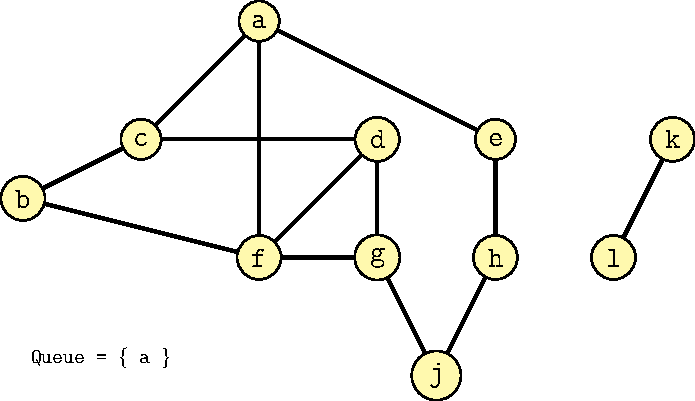
\includegraphics[width=1.0\textwidth,page=1]{errata.pdf}
}
\end{frame}



\begin{frame}{Esempio: Visita errata}

\vspace{-18pt}
\begin{center}
\begin{overprint}
\includegraphics<1|handout:0>[width=1.0\textwidth,page=1]{errata.pdf}
\includegraphics<2|handout:0>[width=1.0\textwidth,page=2]{errata.pdf}
\includegraphics<3|handout:0>[width=1.0\textwidth,page=3]{errata.pdf}
\includegraphics<4|handout:1>[width=1.0\textwidth,page=4]{errata.pdf}
\end{overprint}
\end{center}

\end{frame}

\begin{frame}{Algoritmo generico di attraversamento}
	
\begin{Procedure}
\caption[A]{\textsf{graphTraversal}($\Graph\ G, \Node\ r$)}

$\Set\ S = \setconstructor()$\Comment*{Insieme generico}
$S.\setinsert(r)$\Comment*{Da specificare}
\{ \alert{marca il nodo $r$} \} \;
\While{$S.\getsize()>0$}
{
  $\Node\ u = S.\setremove()$\Comment*{Da specificare}
  \{ \alert{visita il nodo $u$} \}\;
  \ForEach{$v \in G.\adj(u)$}
  {
    \{ \alert{visita l'arco $(u,v)$} \}\;
    \If{$v$ non è ancora stato marcato}
    {
      \{ \alert{marca il nodo $v$} \} \;
      $S.\setinsert(v)$\Comment*{Da specificare}
    }
  }
}
\end{Procedure}

\end{frame}

%%%%%%%%%%%%%%%%%%%%%%%%%%%%%%%%%%%%%%%%%%%%%%%%%%%%%%%%%%%%%%%%%%%%%%%%%%
\section{BFS}
%%%%%%%%%%%%%%%%%%%%%%%%%%%%%%%%%%%%%%%%%%%%%%%%%%%%%%%%%%%%%%%%%%%%%%%%%%

\begin{frame}{Breadth-first search - Obiettivi}

\BB{Visitare i nodi a distanze crescenti dalla sorgente}
\BI
\item Visitare i nodi a distanza $k$ prima di visitare i nodi a distanza $k+1$ 
\EI

\medskip
\BB{Calcolare il cammino più breve da $r$  a tutti gli altri nodi}
\BI
\item Le distanze sono misurate come il numero di archi attraversati
\EI

\medskip
\BB{Generare un \alert{albero breadth-first}}
\BI
\item Generare un albero contenente tutti i nodi raggiungibili da $r$, tale per cui il cammino dalla radice $r$ al nodo $u$ nell'albero corrisponde al cammino più breve da $r$ a $u$ nel grafo.
\EI


\end{frame}

\begin{frame}[shrink=10]{Breadth-first search}

\vspace{-12pt}
\begin{Procedure}
\caption[A]{\bfsproc($\Graph\ G, \Node\ r$)}

$\Queue\ Q = \queueconstructor(\,)$\;
$S.\queueinsert(r)$\;
$\BOOLEAN[\,]\ \mmark = \NEW\ \BOOLEAN[1 \mldots G.\textsf{size}()]$\;
\ForEach{$u \in G.\VV()-\{r\}$}{$\mmark[u] = \FALSE$\;}
$\mmark[r] = \TRUE$\;
\While{\NOT $Q.\queueempty()$}
{
  $\Node\ u = Q.\queueremove()$\;
  \{ \alert{visita il nodo $u$ }\}\;
  \ForEach{$v \in G.\adj(u)$}
  {
    \{ \alert{visita l'arco $(u,v)$} \}\;
    \If{\NOT $\mmark[v]$}
    {
      { $\mmark[v] = \TRUE$ } \;
      $Q.\queueinsert(v)$\;
    }
  }
}
\end{Procedure}

\end{frame}

%%%%%%%%%%%%%%%%%%%%%%%%%%%%%%%%%%%%%%%%%%%%%%%%%%%%%%%%%%%%%%%%%%%%%%%%%%
\subsection{Cammini più brevi}
%%%%%%%%%%%%%%%%%%%%%%%%%%%%%%%%%%%%%%%%%%%%%%%%%%%%%%%%%%%%%%%%%%%%%%%%%%

\begin{frame}{Applicazione BFS: Cammini più brevi}

\vspace{-12pt}
\TwoColsCustom{0.7}{0.25}{
\begin{myboxtitle}[Paul Erdös (1913-1996)]
\BI
\item Matematico
\item 1500+ articoli, 500+ co-autori
\EI
\end{myboxtitle}


\begin{myboxtitle}[Numero di Erdös]
\BI
\item Erdös ha valore $\mathit{erdos} = 0$
\item I co-autori di Erdös hanno $\mathit{erdos} = 1$
\item Se $X$ è co-autore di qualcuno con $\mathit{erdos} = k$ e non è coautore con qualcuno con $\mathit{erdos} < k$, allora $X$ ha $\mathit{erdos} = k+1$
\item Le persone non raggiunte da questa definizione hanno $\mathit{erdos} = +\infty$
\EI
\end{myboxtitle}
}{
\vspace{18pt}
\IG{1.0}{Erdos.jpg}
}

\end{frame}

\begin{frame}{Alberto Montresor, $\mathit{erdos}=4$}
	
\IG{1.0}{erdos-montresor.pdf}
	
\end{frame}

\begin{frame}{Calcolare il numero di Erdös}

\vspace{-12pt}
\begin{Procedure}
\caption[A]{\erdos($\Graph\ G,\ \Node\ r,\ \INTEGER[\,]\ \erdosn,\ \Node[\,]\ \mathit{parent}$)}

$\Queue\ Q = \queueconstructor()$\;
$Q.\queueinsert(r)$\;
\ForEach{$u \in G.\VV()-\{r\}$}{$\erdosn[u] = \infty$}
$\erdosn[r] = 0$\;
$\mathit{parent}[r] = \Nil$\;
\While{\NOT $Q.\queueempty()$}
{
  $\Node\ u = Q.\queueremove()$\;
  \ForEach{$v \in G.\adj(u)$}
  {
    \If(\REMF{Se il nodo $v$ non è stato scoperto}){$\erdosn[v] \Eq \infty$}
    {
      $\erdosn[v] = \erdosn[u]+1$\;
      $\mathit{parent}[v] = u$\;
      $Q.\queueinsert(v)$\;
    }
  }
}
\end{Procedure}

\end{frame}

\begin{frame}{Esempio: Erdös}
\vspace{-12pt}
\centering
\begin{overprint}
\includegraphics<1|handout:0>[width=1.0\textwidth,page=1]{erd.pdf}
\includegraphics<2|handout:0>[width=1.0\textwidth,page=2]{erd.pdf}
\includegraphics<3|handout:0>[width=1.0\textwidth,page=3]{erd.pdf}
\includegraphics<4|handout:0>[width=1.0\textwidth,page=4]{erd.pdf}
\includegraphics<5|handout:0>[width=1.0\textwidth,page=5]{erd.pdf}
\includegraphics<6|handout:0>[width=1.0\textwidth,page=6]{erd.pdf}
\includegraphics<7|handout:0>[width=1.0\textwidth,page=7]{erd.pdf}
\includegraphics<8|handout:0>[width=1.0\textwidth,page=8]{erd.pdf}
\includegraphics<9|handout:0>[width=1.0\textwidth,page=9]{erd.pdf}
\includegraphics<10|handout:0>[width=1.0\textwidth,page=10]{erd.pdf}
\includegraphics<11|handout:1>[width=1.0\textwidth,page=11]{erd.pdf}
\end{overprint}

\end{frame}

\begin{frame}[shrink=10]{Albero BFS (\alert{BFS Tree})}

\vspace{-12pt}
\BIL
\item La visita BFS può essere usata per ottenere il cammino più breve fra due nodi (misurato in numero di archi)
\item "Albero di copertura" con radice $r$
\item Memorizzato in un vettore dei padri $\mathit{parent}$
\EIL

\TwoColsCustom{0.44}{0.54}{
\begin{Procedure}
\caption[A]{$\erdos([\ldots],\ \alert{\Node[\,]\ \mathit{parent}}$)}
[\ldots]\;
\While{\NOT $S.\queueempty()$}
{
  $\Node\ u = S.\queueremove()$\;
  \ForEach{$v \in G.\adj(u)$}
  {
    \If{$\erdosn[v] \Eq \infty$}
    {
      $\erdosn[v] = \erdosn[u]+1$\;
      \alert{$\mathit{parent}[v] = u$}\;
      $S.\queueinsert(v)$\;
    }
  }
}
\end{Procedure}
}{
\begin{Procedure}
\caption[A]{\textsf{printPath}($\Node\ r,\ \Node\ s,\ \Node[\,]\ \mathit{parent}$)}

\uIf{$r \Eq s$}
{
  \textbf{print} $s$
}
\uElseIf{$\mathit{parent}[s] \Eq \Nil$}
{
  \textbf{print} “error”\;
}
\Else
{
  $\textsf{printPath}(r, \mathit{parent}[s], \mathit{parent})$\;
  \textbf{print} $s$\;
}
\end{Procedure}
}

\end{frame}

\begin{frame}{Albero BFS (\alert{BFS Tree})}

\includegraphics[width=1.0\textwidth,page=12]{erd.pdf}

\end{frame}


\begin{frame}{Complessità BFS}

\BB{Complessità: $O(m+n)$}
\BIL
\item Ognuno degli $n$ nodi viene inserito nella coda al massimo una volta 
\item Ogni volta che un nodo viene estratto, tutti i suoi archi vengono analizzati una volta
sola
\item Il numero di archi analizzati è quindi 

\[
  m = \sum_{u \in V} \mathit{out}_d(u) 
\]

dove $\mathit{out}_d(u)$ è l'out-degree del nodo $u$
\EIL

\end{frame}

%%%%%%%%%%%%%%%%%%%%%%%%%%%%%%%%%%%%%%%%%%%%%%%%%%%%%%%%%%%%%%%%%%%%%%%%%%
\section{DFS}
%%%%%%%%%%%%%%%%%%%%%%%%%%%%%%%%%%%%%%%%%%%%%%%%%%%%%%%%%%%%%%%%%%%%%%%%%%


\begin{frame}{Depth-First Search (DFS)}

\BB{Depth-First Search}
\BI
\item Spesso una subroutine della soluzione di altri problemi
\item Utilizzata per esplorare un intero grafo, non solo i nodi 
raggiungibili da una singola sorgente
\EI

\BB{Output}
\BI
\item Invece di un albero, una foresta depth-first $G_f = (V, E_f)$
\item Formata da una collezione di alberi depth-first
\EI

\BB{Struttura dati}
\BI
\item Stack implicito, attraverso la ricorsione
\item Stack esplicito
\EI

\end{frame}



\begin{frame}{Depth-First Search (Ricorsiva, stack implicito)}
	
\begin{Procedure}
\caption[A]{\dfsproc(\Graph $G$, \Node\ $u$, $\BOOLEAN[\,]\ \mmark$)}
  
$\mmark[u] = \TRUE$\;
\{ \alert{visita il nodo $u$ (pre-order)} \}\;
\ForEach{$v \in G.\adj(u)$}
{
  \If{\NOT $\mmark[v]$}
  {
    \{ \alert{visita l'arco $(u,v)$} \}\;
    $\dfsproc(G, v, \mmark)$\; 
  }
}
\{ \alert{visita il nodo $u$ (post-order)} \}\;
\end{Procedure}

\BB{Complessità: $O(m+n)$}

\end{frame}

\begin{frame}{BFS vs DFS}

\begin{columns}[T]
\column{0.55\textwidth}
\BIL
\item Eseguire una DFS basata su chiamate ricorsive può essere rischioso in
grafi molto grandi e connessi
\item \EE possibile che la profondità raggiunta sia troppo grande per la
dimensione dello stack del linguaggio
\item In tali casi, si preferisce utilizzare una BFS oppure una DFS
basata su stack esplicito
\EIL
\column{0.43\textwidth}
\textbf{Stack size in Java}

\smallskip
\IG{1.0}{stack-java.pdf}
\end{columns}
    
\end{frame}

\begin{frame}[shrink=15]{DFS (Iterativa, stack esplicito, pre-order)}

\vspace{-12pt}
\TwoColsCustom{0.58}{0.39}{
\begin{Procedure}
\caption[A]{\dfsproc($\Graph\ G, \Node\ r$)}

$\Stack\ S = \stackconstructor(\,)$\;
$S.\stackpush(r)$\;
$\BOOLEAN[\,]\ \mmark = \NEW\ \BOOLEAN[1 \mldots G.\textsf{size}()]$\;
\ForEach{$u \in G.\VV()$}{$\mmark[u] = \FALSE$\;}
\While{\NOT $S.\stackempty()$}
{
  $\Node\ u = S.\stackpop()$\;
  \If{\NOT $\mmark[u]$}{
    \{ \alert{visita il nodo $u$ (pre-order)} \}\;
    $\mmark[v] = \TRUE$ \;
    \ForEach{$v \in G.\adj(u)$}{
      \{ \alert{visita l'arco $(u,v)$} \}\;
      $S.\stackpush(v)$\;
    }
  }
}
\end{Procedure}
}{
\BB{Note}
\BIL
\item Un nodo può essere inserito nella pila più volte
\item Il controllo se un nodo è già stato visitato viene fatto all'estrazione,
non all'inserimento
\item Complessità $O(m+n)$
 \BI
 \item $O(m)$ visite degli archi
 \item $O(m)$ inserimenti, estrazioni
 \item $O(n)$ visite dei nodi
 \EI
\EIL
}

\end{frame}

\begin{frame}{DFS (Iterativa, stack esplicito, post-order)}

\BB{Visita post-order}
\BIL
\item Quando un nodo viene scoperto:
  \BI
  \item  viene inserito nello stack con il tag \textsf{discovery}
  \EI
\item Quando un nodo viene estratto dalla coda con tag \textsf{discovery}:
  \BI
  \item Viene re-inserito con il tag \textsf{finish}
  \item Tutti i suoi vicini vengono inseriti
  \EI
\item Quando un nodo viene estratto dalla coda con tag \textsf{finish}:
  \BI
  \item Viene effettuata la post-visita
  \EI
\EIL
\end{frame}


%%%%%%%%%%%%%%%%%%%%%%%%%%%%%%%%%%%%%%%%%%%%%%%%%%%%%%%%%%%%%%%%%%%%%%%%%%
\subsection{Componenti connesse}
%%%%%%%%%%%%%%%%%%%%%%%%%%%%%%%%%%%%%%%%%%%%%%%%%%%%%%%%%%%%%%%%%%%%%%%%%%

\begin{frame}{Componenti (fortemente) connesse}

\begin{myboxtitle}[Motivazioni]
\BIL
\item Molti algoritmi che operano sui grafi iniziano decomponendo 
il grafo nel sue componenti connesse.
\item Tali algoritmi sono eseguiti su ognuna delle componenti
\item I risultati sono ricomposti assieme.
\EIL
\end{myboxtitle}

\begin{myboxtitle}[Definizioni]
\BIL
\item \alert{Componenti connesse}, definite su grafi \alert{non orientati}\\
(\emph{Connected components}, CC)
\item \alert{Componenti fortemente connesse}, definite su \alert{grafi orientati}\\
(\emph{Strongly connected components}, SCC)
\EIL
\end{myboxtitle}

\end{frame}

\begin{frame}{Definizioni: Raggiungibilità}

\vspace{-6pt}
\begin{myboxtitle}[Definizione]
Un nodo $v$ è \alert{raggiungibile} da un nodo $u$ se esiste almeno un cammino da $u$ a $v$.
\end{myboxtitle}

\TwoCols{
Il nodo $d$ è raggiungibile dal nodo $a$ e 
viceversa
\medskip
\IG{0.8}{cammino-und.pdf}
}{
Il nodo $d$ è raggiungibile dal nodo $a$, ma 
non viceversa
\medskip
\IG{0.8}{cammino-or2.pdf}
}
\end{frame}



\begin{frame}{Grafi connessi e componenti connesse}

\vspace{-6pt}
\begin{myboxtitle}[Definizioni]
\BIL
\item Un grafo non orientato $G=(V,E)$ è \alert{connesso} $\Leftrightarrow$ ogni
suo nodo è raggiungibile da ogni altro suo nodo
\item Un grafo $G'=(V',E')$ è una \alert{componente connessa} di $G$ $\Leftrightarrow$ $G'$ è un sottografo connesso e massimale di $G$
\EIL

\TwoColsCustom{0.52}{0.45}{
\BIL
\item $G'$ è un \alert{sottografo} di $G$ ($G' \subseteq G$) $\Leftrightarrow$ $V' \subseteq V$ e $E'
\subseteq E$
\item $G'$ è \alert{massimale} $\Leftrightarrow$ non esiste nessun altro sottografo $G''$ di $G$ tale che $G''$
è connesso e più grande di $G'$ (i.e. $G' \subseteq G'' \subseteq G$)
\EIL
}{
\vspace{-12pt}
\IG{1.0}{cc.pdf}
}
\end{myboxtitle}


\end{frame}

\begin{frame}{Applicazione DFS: Componenti connesse}

\vspace{-6pt}
\begin{myboxtitle}[Problema]
\BI
\item Verificare se un grafo è connesso oppure no
\item Identificare le sue componenti connesse
\EI
\end{myboxtitle}

\pause
\begin{myboxtitle}[Soluzione]
\BI
\item Un grafo è connesso se, al termine della DFS, tutti i nodi sono marcati
\item Altrimenti, la visita deve ricominciare da capo da un nodo non marcato, identificando una nuova componente del grafo
\EI
\end{myboxtitle}

\begin{myboxtitle}[Strutture dati]
\BI
\item Un vettore $\components$, che contiene gli identificatori delle componenti
\item $\components[u]$ è l'identificatore della c.c. a cui appartiene $u$
\EI
\end{myboxtitle}

\end{frame}


\begin{frame}{Applicazione DFS: Componenti connesse}

\vspace{-12pt}
\begin{columns}[T]
\column{0.45\textwidth}
\begin{Procedure}
\caption[A]{$\INTEGER[\,]$ \connectedcomponents(\Graph $G$)}
$\INTEGER[\,]\ \components = \NEW\ \INTEGER[1 \mldots G.\textsf{size}()]$\;
\ForEach{$u \in G.\VV()$}
{
  $\components[u] = 0$
}
\INTEGER\ $\mathit{counter} = 0$\;
\ForEach{$u \in G.\VV()$}
{
  \If{$\components[u] \Eq 0$}
  {
    $\mathit{counter} = \mathit{counter}+1$\;
    $\ccdfs(G, \mathit{counter}, u, \components)$\;
  }
}
\Return \components\;
\end{Procedure}
\column{0.51\textwidth}
\begin{Procedure}
\caption[A]{\ccdfs(\Graph $G$, \INTEGER\ $\mathit{counter}$, \Node\ $u$, $\INTEGER[\,]\ \components$)}
$\components[u] = \mathit{counter}$\;
\ForEach{$v \in G.\adj(u)$}
{
  \If{$\components[v] \Eq 0$}{$\ccdfs(G, \mathit{counter}, v, \components)$}
}
\end{Procedure}
\end{columns}
\end{frame}



\begin{frame}{Esempio: Componenti connesse}

\centering
\begin{overprint}
\includegraphics<1|handout:0>[width=1.00\textwidth,page=1]{ccex-anim.pdf}
\includegraphics<2|handout:0>[width=1.00\textwidth,page=2]{ccex-anim.pdf}
\includegraphics<3|handout:0>[width=1.00\textwidth,page=3]{ccex-anim.pdf}
\includegraphics<4|handout:0>[width=1.00\textwidth,page=4]{ccex-anim.pdf}
\includegraphics<5|handout:0>[width=1.00\textwidth,page=5]{ccex-anim.pdf}
\includegraphics<6|handout:0>[width=1.00\textwidth,page=6]{ccex-anim.pdf}
\includegraphics<7|handout:0>[width=1.00\textwidth,page=7]{ccex-anim.pdf}
\includegraphics<8|handout:0>[width=1.00\textwidth,page=8]{ccex-anim.pdf}
\includegraphics<9|handout:0>[width=1.00\textwidth,page=9]{ccex-anim.pdf}
\includegraphics<10|handout:0>[width=1.00\textwidth,page=10]{ccex-anim.pdf}
\includegraphics<11|handout:0>[width=1.00\textwidth,page=11]{ccex-anim.pdf}
\includegraphics<12|handout:0>[width=1.00\textwidth,page=12]{ccex-anim.pdf}
\includegraphics<13|handout:0>[width=1.00\textwidth,page=13]{ccex-anim.pdf}
\includegraphics<14|handout:0>[width=1.00\textwidth,page=14]{ccex-anim.pdf}
\includegraphics<15|handout:0>[width=1.00\textwidth,page=15]{ccex-anim.pdf}
\includegraphics<16|handout:0>[width=1.00\textwidth,page=16]{ccex-anim.pdf}
\includegraphics<17|handout:0>[width=1.00\textwidth,page=17]{ccex-anim.pdf}
\includegraphics<18|handout:0>[width=1.00\textwidth,page=18]{ccex-anim.pdf}
\includegraphics<19|handout:0>[width=1.00\textwidth,page=19]{ccex-anim.pdf}
\includegraphics<20|handout:0>[width=1.00\textwidth,page=20]{ccex-anim.pdf}
\includegraphics<21|handout:0>[width=1.00\textwidth,page=21]{ccex-anim.pdf}
\includegraphics<22|handout:0>[width=1.00\textwidth,page=22]{ccex-anim.pdf}
\includegraphics<23|handout:0>[width=1.00\textwidth,page=23]{ccex-anim.pdf}
\includegraphics<24|handout:0>[width=1.00\textwidth,page=24]{ccex-anim.pdf}
\includegraphics<25|handout:0>[width=1.00\textwidth,page=25]{ccex-anim.pdf}
\includegraphics<26|handout:0>[width=1.00\textwidth,page=26]{ccex-anim.pdf}
\includegraphics<27|handout:0>[width=1.00\textwidth,page=27]{ccex-anim.pdf}
\includegraphics<28|handout:0>[width=1.00\textwidth,page=28]{ccex-anim.pdf}
\includegraphics<29|handout:0>[width=1.00\textwidth,page=29]{ccex-anim.pdf}
\includegraphics<30|handout:0>[width=1.00\textwidth,page=30]{ccex-anim.pdf}
\includegraphics<31|handout:0>[width=1.00\textwidth,page=31]{ccex-anim.pdf}
\includegraphics<32|handout:0>[width=1.00\textwidth,page=32]{ccex-anim.pdf}
\includegraphics<33|handout:0>[width=1.00\textwidth,page=33]{ccex-anim.pdf}
\includegraphics<34|handout:0>[width=1.00\textwidth,page=34]{ccex-anim.pdf}
\includegraphics<35|handout:1>[width=1.00\textwidth,page=35]{ccex-anim.pdf}
v\end{overprint}

\end{frame}

%%%%%%%%%%%%%%%%%%%%%%%%%%%%%%%%%%%%%%%%%%%%%%%%%%%%%%%%%%%%%%%%%%%%%%%%%%
\subsection{Grafi aciclici non orientati}
%%%%%%%%%%%%%%%%%%%%%%%%%%%%%%%%%%%%%%%%%%%%%%%%%%%%%%%%%%%%%%%%%%%%%%%%%%

%-------------------------------------------------------------------------
\begin{frame}{Definizioni: Ciclo}
	
\vspace{-6pt}
\begin{myboxtitle}[Ciclo (cycle)]
In un grafo non orientato $G=(V,E)$, un \alert{ciclo} $C$ di lunghezza $k > 2$ è una sequenza di nodi $u_0, u_1, \ldots, u_k$ tale che $(u_i, u_{i+1} \in E)$ per $0 \leq i \leq k-1$ e $u_0 = u_k$.
\end{myboxtitle}

\TwoCols{
\vspace{-12pt}
\IG{1.0}{ciclo-non.pdf}
}{
\medskip
$k > 2$ esclude cicli banali composti da coppie di archi $(u,v)$ e $(v,u)$, che sono onnipresenti nei grafi non orientati.
}

\end{frame}


%-------------------------------------------------------------------------
\begin{frame}{Definizioni: Grafo aciclico}

\vspace{-6pt}
\begin{columns}[T]
\column{0.55\textwidth}

\begin{myboxtitle}[Grafo aciclico]
Un grafo non orientato che non contiene cicli è detto \alert{aciclico}.
\end{myboxtitle}
\column{0.40\textwidth}
\vspace{-12pt}
\IG{1.0}{acyclic-und.pdf}
\end{columns}

\bigskip
\begin{myboxtitle}[Problema]
Dato un grafo non orientato $G$, scrivere un algoritmo che restituisca \textbf{true} se $G$ contiene un ciclo, \textbf{false}
altrimenti.
\end{myboxtitle}

\end{frame}

%-------------------------------------------------------------------------
\begin{frame}[shrink=10]{Applicazione DFS: Grafo non orientato aciclico}

\large
\begin{Procedure}
\caption[A]{$\BOOLEAN\ \textsf{hasCycleRec}(\Graph\ G,\ \Node\ u, \Node\ p, \BOOLEAN[\,]\ \mmark)$}

$\mmark[u] = \TRUE$\;
\ForEach{$v \in G.\adj(u) - \{ p \}$}
{
  \uIf{$\mmark[v]$}
  {
    \Return \TRUE\;
  }
  \ElseIf{$\textsf{hasCycleRec}(G, v, u, \mmark)$}
  {
    \Return \TRUE\;
  }
}
\Return \FALSE\;
\end{Procedure}

\end{frame}

%-------------------------------------------------------------------------
\begin{frame}[shrink=10]{Applicazione DFS: Grafo non orientato aciclico}

\large
\begin{Procedure}
\caption[A]{$\BOOLEAN\ \textsf{hasCycle}(\Graph\ G)$}
$\BOOLEAN[\,]\ \mmark = \NEW\ \BOOLEAN[1 \mldots G.\textsf{size}()]$\;
\ForEach{$u \in G.\VV()$}{
  $\mmark[u] = \FALSE$\;
}
\ForEach{$u \in G.\VV()$}{
  \If{$\NOT\ \mmark[u]$}{
    \If{$\textsf{hasCyclerec}(G, u, \NULL, \mmark)$}{
      \Return \TRUE\;
    }
  }
}
\Return \FALSE\;
\end{Procedure}

\end{frame}


%-------------------------------------------------------------------------
\begin{frame}{Definizioni: Ciclo}
	
\vspace{-6pt}
\begin{myboxtitle}[Ciclo (cycle)]
In un grafo orientato $G=(V,E)$, un \alert{ciclo} $C$ di lunghezza $k \geq 2$ è una sequenza di nodi $u_0, u_1, \ldots, u_k$ tale che $(u_i, u_{i+1} \in E)$ per $0 \leq i \leq k-1$ e $u_0 = u_k$.
\end{myboxtitle}

\TwoCols{
\vspace{-12pt}
\IG{1.0}{ciclo.pdf}
}{
\medskip
\alert{Esempio}: $a, b, c, e, d, a$ è un cammino nel grafo di lunghezza $5$

\medskip
Note: un ciclo è detto \alert{semplice} se tutti i suoi nodi sono distinti
(ad esclusione del primo e dell'ultimo)
}

\end{frame}

%-------------------------------------------------------------------------
\begin{frame}{Definizioni: Grafo orientato aciclico (DAG)}

\vspace{-6pt}
\begin{columns}[T]
\column{0.48\textwidth}
\begin{myboxtitle}[DAG]
Un grafo orientato che non contiene cicli è detto \alert{DAG} (\alert{directed acyclic graph}).
\end{myboxtitle}

\bigskip
\begin{myboxtitle}[Grafo ciclico]
Un grafo è \alert{ciclico} se contiene un ciclo.
\end{myboxtitle}
    
\column{0.48\textwidth}
\vspace{-12pt}
\IG{0.9}{acyclic.pdf}

\end{columns}
\end{frame}

\begin{frame}{Applicazione DFS: Grafo orientato aciclico}

\begin{myboxtitle}[Problema]
Dato un grafo orientato $G$, scrivere un algoritmo che restituisca \textbf{true} se $G$ contiene un ciclo, \textbf{false}
altrimenti.
\end{myboxtitle}

\begin{myboxtitle}[Problema]
Riuscite a concepire un grafo orientato per cui l'algoritmo appena visto 
non si comporta correttamente?
\end{myboxtitle}

\begin{center}
\begin{overprint}[0.4\textwidth]
\includegraphics<2|handout:0>[width=0.4\textwidth,page=1]{acyclic-error.pdf}
\includegraphics<3|handout:0>[width=0.4\textwidth,page=2]{acyclic-error.pdf}
\includegraphics<4|handout:0>[width=0.4\textwidth,page=3]{acyclic-error.pdf}
\includegraphics<5|handout:0>[width=0.4\textwidth,page=4]{acyclic-error.pdf}
\includegraphics<6|handout:0>[width=0.4\textwidth,page=5]{acyclic-error.pdf}
\end{overprint}
\end{center}

\end{frame}


%%%%%%%%%%%%%%%%%%%%%%%%%%%%%%%%%%%%%%%%%%%%%%%%%%%%%%%%%%%%%%%%%%%%%%%%%%
\subsection{Classificazione degli archi}
%%%%%%%%%%%%%%%%%%%%%%%%%%%%%%%%%%%%%%%%%%%%%%%%%%%%%%%%%%%%%%%%%%%%%%%%%%


\begin{frame}{Classificazione degli archi}

\vspace{-6pt}
\begin{myboxtitle}[Albero di copertura DFS]
Ogni volta che si esamina un arco da un nodo marcato ad un nodo non marcato, tale arco viene \alert{arco dell'albero}
\end{myboxtitle}

\TwoColsCustom{0.6}{0.36}{
\vspace{-6pt}
\BB{Gli archi $(u,v)$ non inclusi nell'albero possono essere divisi 
in tre categorie}
\BIL
\item Se $u$ è un antenato di $v$ in $T$, 
$(u,v)$ è detto {\color{violet} arco in avanti}
\item Se $u$ è un discendente di $v$ in $T$, 
$(u,v)$ è detto {\color{brown} arco all'indietro}
\item Altrimenti, viene detto {\color{blue} arco di attraversamento}
\EIL
}{
\vspace{-18pt}
\IG{0.65}{schema.pdf}
}

\end{frame}

\begin{frame}[shrink=15]{DFS Schema}

\vspace{-12pt}
\TwoColsCustom{0.7}{0.28}{
\begin{Procedure}
\caption[A]{\dfsschema(\Graph $G$, \Node\ $u$, \INTEGER\ \&$\orologio$, $\INTEGER[\,]\ \ddt$, $\INTEGER[\,]\ \dft$)}
\{ visita il nodo $u$ (pre-order) \} \;
$\orologio = \orologio + 1$;~~ $\ddt[u] = \orologio$\;
\ForEach{$v \in G.\adj(u)$}
{
  \{ visita l'arco $(u,v)$ (qualsiasi) \} \;
  \uIf{$\ddt[v] \Eq 0$}
  {
		\color{red}{\{ visita l'arco $(u,v)$ (albero) \}} \;
        $\dfsschema(G, v, \orologio, \ddt, \dft)$\; 
  }
  \uElseIf{$\ddt[u]>\ddt[v]$ \AND $\dft[v] \Eq 0$}{
		\color{brown}{\{ visita l'arco $(u,v)$ (indietro) \}} \;
  }
  \uElseIf{$\ddt[u]<\ddt[v]$ \AND $\dft[v] \neq 0$}{
		\color{violet}{\{ visita l'arco $(u,v)$ (avanti) \}} \;
  }
  \Else
  {
		\color{blue}{\{ visita l'arco $(u,v)$ (attraversamento) \}} \;
  }
}
\{ visita il nodo $u$ (post-order) \} \;
$\orologio = \orologio + 1$;~~
$\dft[u] = \orologio$\;
\end{Procedure}
	}{
\vspace{24pt}
\BIL
\item $\orologio$: contatore
\item $\ddt$: \alert{discovery time} (tempo di scoperta)
\item $\dft$: \alert{finish time} (tempo di fine)
\EIL
	
}
\end{frame}

% \begin{frame}{Esempio: DFS Schema su grafo non orientato}
%
% \centering
% \begin{overprint}
% \includegraphics<1|handout:0>[width=1.00\textwidth,page=1]{dfs-schema.pdf}
% \includegraphics<2|handout:0>[width=1.00\textwidth,page=2]{dfs-schema.pdf}
% \includegraphics<3|handout:0>[width=1.00\textwidth,page=3]{dfs-schema.pdf}
% \includegraphics<4|handout:0>[width=1.00\textwidth,page=4]{dfs-schema.pdf}
% \includegraphics<5|handout:0>[width=1.00\textwidth,page=5]{dfs-schema.pdf}
% \includegraphics<6|handout:0>[width=1.00\textwidth,page=6]{dfs-schema.pdf}
% \includegraphics<7|handout:0>[width=1.00\textwidth,page=7]{dfs-schema.pdf}
% \includegraphics<8|handout:0>[width=1.00\textwidth,page=8]{dfs-schema.pdf}
% \includegraphics<9|handout:0>[width=1.00\textwidth,page=9]{dfs-schema.pdf}
% \includegraphics<10|handout:0>[width=1.00\textwidth,page=10]{dfs-schema.pdf}
% \includegraphics<11|handout:0>[width=1.00\textwidth,page=11]{dfs-schema.pdf}
% \includegraphics<12|handout:0>[width=1.00\textwidth,page=12]{dfs-schema.pdf}
% \includegraphics<13|handout:0>[width=1.00\textwidth,page=13]{dfs-schema.pdf}
% \includegraphics<14|handout:0>[width=1.00\textwidth,page=14]{dfs-schema.pdf}
% \includegraphics<15|handout:0>[width=1.00\textwidth,page=15]{dfs-schema.pdf}
% \includegraphics<16|handout:0>[width=1.00\textwidth,page=16]{dfs-schema.pdf}
% \includegraphics<17|handout:0>[width=1.00\textwidth,page=17]{dfs-schema.pdf}
% \includegraphics<18|handout:0>[width=1.00\textwidth,page=18]{dfs-schema.pdf}
% \includegraphics<19|handout:0>[width=1.00\textwidth,page=19]{dfs-schema.pdf}
% \includegraphics<20|handout:0>[width=1.00\textwidth,page=20]{dfs-schema.pdf}
% \includegraphics<21|handout:0>[width=1.00\textwidth,page=21]{dfs-schema.pdf}
% \includegraphics<22|handout:0>[width=1.00\textwidth,page=22]{dfs-schema.pdf}
% \includegraphics<23|handout:0>[width=1.00\textwidth,page=23]{dfs-schema.pdf}
% \includegraphics<24|handout:0>[width=1.00\textwidth,page=24]{dfs-schema.pdf}
% \includegraphics<25|handout:0>[width=1.00\textwidth,page=25]{dfs-schema.pdf}
% \includegraphics<26|handout:0>[width=1.00\textwidth,page=26]{dfs-schema.pdf}
% \includegraphics<27|handout:0>[width=1.00\textwidth,page=27]{dfs-schema.pdf}
% \includegraphics<28|handout:0>[width=1.00\textwidth,page=28]{dfs-schema.pdf}
% \includegraphics<29|handout:0>[width=1.00\textwidth,page=29]{dfs-schema.pdf}
% \includegraphics<30|handout:1>[width=1.00\textwidth,page=30]{dfs-schema.pdf}
% \end{overprint}
%
% \end{frame}



\begin{frame}{DFS Schema}

\vspace{-18pt}
\TwoColsCustom{0.65}{0.33}{
\small
\begin{Procedure}
\caption[A]{\footnotesize \dfsschema(\Graph $G$, \Node\ $u$, \INTEGER\ \&$\orologio$, $\INTEGER[\,]\ \ddt$, $\INTEGER[\,]\ \dft$)}
$\orologio = \orologio + 1$;~~ $\ddt[u] = \orologio$\;
\ForEach{$v \in G.\adj(u)$}
{
  \uIf{$\ddt[v] \Eq 0$}
  {
		\color{red}{\{ visita l'arco $(u,v)$ (albero) \}} \;
        $\dfsschema(G, v, \orologio, \ddt, \dft)$\; 
  }
  \uElseIf{$\ddt[u]>\ddt[v]$ \AND $\dft[v] \Eq 0$}{
		\color{brown}{\{ visita l'arco $(u,v)$ (indietro) \}} \;
  }
  \uElseIf{$\ddt[u]<\ddt[v]$ \AND $\dft[v] \neq 0$}{
		\color{violet}{\{ visita l'arco $(u,v)$ (avanti) \}} \;
  }
  \Else
  {
		\color{blue}{\{ visita l'arco $(u,v)$ (attraversamento) \}} \;
  }
}
$\orologio = \orologio + 1$;~~
$\dft[u] = \orologio$\;
\end{Procedure}
	}{
\vspace{12pt}
\begin{overprint}
\includegraphics<1|handout:0>[width=1.0\textwidth,page=1]{schema-esempio.pdf}	
\includegraphics<2|handout:0>[width=1.0\textwidth,page=2]{schema-esempio.pdf}	
\includegraphics<3|handout:0>[width=1.0\textwidth,page=3]{schema-esempio.pdf}	
\includegraphics<4|handout:0>[width=1.0\textwidth,page=4]{schema-esempio.pdf}	
\includegraphics<5|handout:0>[width=1.0\textwidth,page=5]{schema-esempio.pdf}	
\includegraphics<6|handout:0>[width=1.0\textwidth,page=6]{schema-esempio.pdf}	
\includegraphics<7|handout:0>[width=1.0\textwidth,page=7]{schema-esempio.pdf}	
\includegraphics<8|handout:0>[width=1.0\textwidth,page=8]{schema-esempio.pdf}	
\includegraphics<9|handout:0>[width=1.0\textwidth,page=9]{schema-esempio.pdf}	
\includegraphics<10|handout:0>[width=1.0\textwidth,page=10]{schema-esempio.pdf}	
\includegraphics<11|handout:0>[width=1.0\textwidth,page=11]{schema-esempio.pdf}	
\includegraphics<12|handout:0>[width=1.0\textwidth,page=12]{schema-esempio.pdf}	
\includegraphics<13|handout:0>[width=1.0\textwidth,page=13]{schema-esempio.pdf}	
\includegraphics<14|handout:0>[width=1.0\textwidth,page=14]{schema-esempio.pdf}	
\includegraphics<15|handout:0>[width=1.0\textwidth,page=15]{schema-esempio.pdf}	
\includegraphics<16|handout:0>[width=1.0\textwidth,page=16]{schema-esempio.pdf}	
\includegraphics<17|handout:0>[width=1.0\textwidth,page=17]{schema-esempio.pdf}	
\includegraphics<18|handout:1>[width=1.0\textwidth,page=18]{schema-esempio.pdf}	
\end{overprint}
}
\end{frame}

\begin{frame}{Classificazione degli archi}

\vspace{-6pt}
\begin{myboxtitle}[Perchè classificare gli archi?]
Possiamo dimostrare proprietà sul tipo degli archi e usare queste proprietà
per costruire algoritmi migliori
\end{myboxtitle}

\begin{myboxtitle}[Teorema]
Data una visita DFS di un grafo  $G=(V,E)$, per ogni coppia di nodi 
$u,v \in V$, solo una delle condizioni seguenti è vera:
\BI 
\item Gli intervalli $[\ddt[u], \dft[u]]$ e $[\ddt[v], \dft[v]]$ sono 
non-sovrapposti; \\
\alert{$u,v$ non sono discendenti l'uno dell'altro} nella foresta DF
\item L'intervallo $[\ddt[u], \dft[u]]$ è contenuto in $[\ddt[v], \dft[v]]$;\\
\alert{$u$ è un discendente di $v$} in un albero DF
\item L'intervallo $[\ddt[v], \dft[v]]$ è contenuto in $[\ddt[u], \dft[u]]$;\\
\alert{$v$ è un discendente di $u$} in un albero DF
\EI
\end{myboxtitle}

\end{frame}


%%%%%%%%%%%%%%%%%%%%%%%%%%%%%%%%%%%%%%%%%%%%%%%%%%%%%%%%%%%%%%%%%%%%%%%%%%
\subsection{Grafi aciclici orientati}
%%%%%%%%%%%%%%%%%%%%%%%%%%%%%%%%%%%%%%%%%%%%%%%%%%%%%%%%%%%%%%%%%%%%%%%%%%


\begin{frame}{Teoria}

\vspace{-6pt}
\begin{myboxtitle}[Teorema]
Un grafo orientato è aciclico $\Leftrightarrow$ non esistono archi all'indietro nel grafo.
\end{myboxtitle}

\begin{myboxtitle}[Dimostrazione]
\begin{itemize}
\item {\bf se}: Se
	esiste un ciclo, sia $u$ il primo nodo del ciclo che viene visitato e sia
	$(v,u)$ un arco del ciclo. Il cammino che connette $u$ ad $v$ verrà prima o
	poi visitato, e da $v$ verrà scoperto l'arco all'indietro $(v,u)$.
\item 
  {\bf solo se}: Se
esiste un arco all'indietro $(u,v)$, dove $v$ è un antenato di $u$, allora
esiste un cammino da $v$ a $u$ e un arco da $u$ a $v$, ovvero un ciclo.
\end{itemize}
\end{myboxtitle}

\end{frame}

\begin{frame}{Applicazione DFS: DAG}

\begin{Procedure}
\caption[A]{$\BOOLEAN\ \textsf{hasCycle}(\Graph\ G,\ \Node\ u, \INTEGER\ \&\orologio, \INTEGER[\,]\ \ddt, \INTEGER[\,]\ \dft)$}

$\orologio = \orologio + 1$;~~
$\ddt[u] = \orologio$\;
\ForEach{$v \in G.\adj(u)$}
{
  \uIf{$\ddt[v] \Eq 0$}
  {
    \If{$\textsf{hasCycle}(G, v, \orologio, \ddt, \dft)$}{\Return \TRUE} 
  }
  \ElseIf{$\ddt[u]>\ddt[v]$ \AND $\dft[v] \Eq 0$}
  {
    \Return \TRUE\;
  }
}
$\orologio = \orologio + 1$;~~
$\dft[u] = \orologio$\;
\Return \FALSE\;
\end{Procedure}

\end{frame}

\begin{frame}{Applicazione DFS: DAG}

\begin{center}
\begin{overprint}[0.5\textwidth]
\onslide<1|handout:0>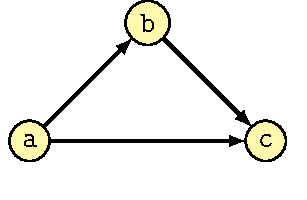
\includegraphics[width=1.0\textwidth,page=1]{acyclic-schema.pdf}
\onslide<2|handout:0>\includegraphics[width=1.0\textwidth,page=2]{acyclic-schema.pdf}
\onslide<3|handout:0>\includegraphics[width=1.0\textwidth,page=3]{acyclic-schema.pdf}
\onslide<4|handout:0>\includegraphics[width=1.0\textwidth,page=4]{acyclic-schema.pdf}
\onslide<5|handout:0>\includegraphics[width=1.0\textwidth,page=5]{acyclic-schema.pdf}
\onslide<6|handout:0>\includegraphics[width=1.0\textwidth,page=6]{acyclic-schema.pdf}
\onslide<7|handout:0>\includegraphics[width=1.0\textwidth,page=7]{acyclic-schema.pdf}
\onslide<8|handout:0>\includegraphics[width=1.0\textwidth,page=8]{acyclic-schema.pdf}
\onslide<9|handout:0>\includegraphics[width=1.0\textwidth,page=9]{acyclic-schema.pdf}
\onslide<10|handout:1>\includegraphics[width=1.0\textwidth,page=10]{acyclic-schema.pdf}
\end{overprint}

\bigskip
\begin{tabular}{rl}
Arco dell'albero & \color{red}{$\ddt[v] \Eq 0$}\\
Arco all'indietro: & \color{brown}{$\ddt[u]>\ddt[v]$ \AND $\dft[v] = 0$}\\
Arco in avanti: & \color{violet}{$\ddt[u]<\ddt[v]$ \AND $\dft[v] \neq 0$} \\
Arco attraversamento: & \color{blue}{altrimenti}
\end{tabular}
\end{center}

\end{frame}

\begin{frame}{Applicazione DFS: DAG}

Non viene individuato nessun arco all'indietro, quindi tutte le chiamate ricorsive arriveranno al termine e ritorneranno \FALSE.


\begin{Procedure}
\caption[A]{$\BOOLEAN\ \textsf{hasCycle}(\Graph\ G,\ \Node\ u, \INTEGER\ \&\orologio, \INTEGER[\,]\ \ddt, \INTEGER[\,]\ \dft)$}

$\orologio = \orologio + 1$;~~
$\ddt[u] = \orologio$\;
\ForEach{$v \in G.\adj(u)$}
{
  \uIf{$\ddt[v] \Eq 0$}
  {
    \If{$\textsf{hasCycle}(G, v, \orologio, \ddt, \dft)$}{\Return \TRUE} 
  }
  \ElseIf{$\ddt[u]>\ddt[v]$ \AND $\dft[v] \Eq 0$}
  {
    \Return \TRUE\;
  }
}
$\orologio = \orologio + 1$;~~
$\dft[u] = \orologio$\;
\alert{\Return \FALSE}\;
\end{Procedure}

\end{frame}

\begin{frame}{Applicazione DFS: DAG}

\begin{center}
\begin{overprint}[0.5\textwidth]
\onslide<1|handout:0>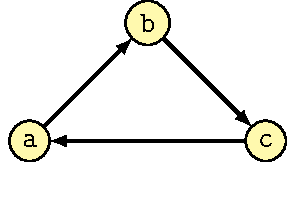
\includegraphics[width=1.0\textwidth,page=1]{acyclic-schema-ciclo.pdf}
\onslide<2|handout:0>\includegraphics[width=1.0\textwidth,page=2]{acyclic-schema-ciclo.pdf}
\onslide<3|handout:0>\includegraphics[width=1.0\textwidth,page=3]{acyclic-schema-ciclo.pdf}
\onslide<4|handout:0>\includegraphics[width=1.0\textwidth,page=4]{acyclic-schema-ciclo.pdf}
\onslide<5|handout:0>\includegraphics[width=1.0\textwidth,page=5]{acyclic-schema-ciclo.pdf}
\onslide<6|handout:0>\includegraphics[width=1.0\textwidth,page=6]{acyclic-schema-ciclo.pdf}
\onslide<7|handout:1>\includegraphics[width=1.0\textwidth,page=7]{acyclic-schema-ciclo.pdf}
\end{overprint}

\bigskip
\begin{tabular}{rl}
Arco dell'albero & \color{red}{$\ddt[v] \Eq 0$}\\
Arco all'indietro: & \color{brown}{$\ddt[u]>\ddt[v]$ \AND $\dft[v] = 0$}\\
Arco in avanti: & \color{violet}{$\ddt[u]<\ddt[v]$ \AND $\dft[v] \neq 0$} \\
Arco attraversamento: & \color{blue}{altrimenti}
\end{tabular}
\end{center}

\end{frame}

\begin{frame}{Applicazione DFS: DAG}

Viene individuato un arco all'indietro, che causa la restituzione di \TRUE in una chiamata e la conseguente restituzione di \TRUE da parte di tutte le chiamate ricorsive precedenti.

\begin{Procedure}
\caption[A]{$\BOOLEAN\ \textsf{hasCycle}(\Graph\ G,\ \Node\ u, \INTEGER\ \&\orologio, \INTEGER[\,]\ \ddt, \INTEGER[\,]\ \dft)$}

$\orologio = \orologio + 1$;~~
$\ddt[u] = \orologio$\;
\ForEach{$v \in G.\adj(u)$}
{
  \uIf{$\ddt[v] \Eq 0$}
  {
    \If{$\textsf{hasCycle}(G, v, \orologio, \ddt, \dft)$}{\alert{\Return \TRUE}} 
  }
  \ElseIf{$\ddt[u]>\ddt[v]$ \AND $\dft[v] \Eq 0$}
  {
    \alert{\Return \TRUE}\;
  }
}
$\orologio = \orologio + 1$;~~
$\dft[u] = \orologio$\;
\Return \FALSE\;
\end{Procedure}

\end{frame}


%%%%%%%%%%%%%%%%%%%%%%%%%%%%%%%%%%%%%%%%%%%%%%%%%%%%%%%%%%%%%%%%%%%%%%%%%%
\subsection{Ordinamento topologico}
%%%%%%%%%%%%%%%%%%%%%%%%%%%%%%%%%%%%%%%%%%%%%%%%%%%%%%%%%%%%%%%%%%%%%%%%%%

\begin{frame}{Ordinamento topologico}

\vspace{-6pt}
\begin{myboxtitle}[Definizione]
Dato un DAG $G$, un \alert{ordinamento topologico} di $G$ è un ordinamento lineare dei suoi nodi tale che se $(u,v) \in E$, allora $u$ appare prima di $v$ nell'ordinamento.
\end{myboxtitle}
    
\BI
\item Esistono più ordinamenti topologici
\item Se il grafo contiene un ciclo, non esiste un ordinamento topologico.
\EI

\IG{0.8}{top-sort1.pdf}

\end{frame}

\begin{frame}{Ordinamento topologico}

\begin{myboxtitle}[Problema]
Scrivere un algoritmo che prende in input un DAG e ritorna un ordinamento
topologico per esso.
\end{myboxtitle}

\pause
\begin{myboxtitle}[Naive solution]
\BIL
\item Trovare un nodo senza archi entranti
\item Aggiungere questo nodo nell'ordinamento e rimuoverlo, insieme a tutti i suoi archi
\item Ripetere questa procedura fino a quando tutti i nodi sono stati rimossi
\EIL
\end{myboxtitle}

\BB{Arthur B. Kahn. \emph{Topological sorting of large networks}.  Communications of the ACM, 5(11):558–562, 1962.}
    
\end{frame}

\begin{frame}{Ordinamento topologico - Algoritmi naive}

\vspace{-12pt}
\IG{0.8}{top-sort2.pdf}

\end{frame}

\begin{frame}{Ordinamento topologico basato su DFS}

\vspace{-6pt}
\BB{Algoritmo}
\BI
\item Eseguire una DFS nel quale l'operazione di visita consiste nell'aggiungere il nodo in testa ad una lista, "at finish time" (post-ordine)
\item Restituire la lista così ottenuta.
\EI

\medskip
\BB{Output}
\BI
\item La sequenza dei nodi, ordinati per tempo decrescente di fine.
\EI

\medskip
\BB{Perchè funziona?}
\pause
\BI
\item Quando un nodo è "finito", tutti i suoi discendenti sono stati scoperti e aggiunti alla lista. Aggiungendolo in testa alla lista, il nodo è in ordine corretto.
\EI

\end{frame}

\begin{frame}[shrink=10]{Ordinamento topologico - L'algoritmo}

\vspace{-12pt}
\begin{Procedure}
\caption[A]{\Stack\ \topsort(\Graph $G$)}
$\Stack\ S = \stackconstructor()$\;
$\BOOLEAN[\,]\ \mmark = \BOOLEAN[1 \mldots G.\textsf{size}()]$\;
\lForEach{$u \in G.\VV()$}{$\mmark[u] = \FALSE$}
\ForEach{$u \in G.\VV()$}
{
  \If{\NOT\ $\mmark[u]$}
  {
    $\topsortdfs(G, u, \mmark, S)$\;
  }
}
\Return $S$\;
\end{Procedure}

\vspace{-16pt}
\begin{Procedure}
\caption[A]{\topsortdfs(\Graph $G$, \Node\ $u$, $\BOOLEAN[\,]\ \mmark$, \Stack $S$)}
$\mmark[u] = \TRUE$\;
\ForEach{$v \in G.\adj(u)$}
{
  \If{\NOT $\mmark[v]$}{$\topsortdfs(G, v, \mmark, S)$}
}
$S.\stackpush(u)$\;
\end{Procedure}

\end{frame}

\begin{frame}{Ordinamento topologico -- Esempio}

\vspace{-24pt}
\begin{columns}[T]
\column{0.45\textwidth}
\begin{overprint}
\includegraphics<1|handout:0>[width=\textwidth,page=1]{topsort.pdf}
\includegraphics<2|handout:0>[width=\textwidth,page=2]{topsort.pdf}
\includegraphics<3|handout:0>[width=\textwidth,page=3]{topsort.pdf}
\includegraphics<4|handout:0>[width=\textwidth,page=4]{topsort.pdf}
\includegraphics<5|handout:0>[width=\textwidth,page=5]{topsort.pdf}
\includegraphics<6|handout:0>[width=\textwidth,page=6]{topsort.pdf}
\includegraphics<7|handout:0>[width=\textwidth,page=7]{topsort.pdf}
\includegraphics<8|handout:0>[width=\textwidth,page=8]{topsort.pdf}
\includegraphics<9|handout:0>[width=\textwidth,page=9]{topsort.pdf}
\includegraphics<10|handout:0>[width=\textwidth,page=10]{topsort.pdf}
\includegraphics<11|handout:0>[width=\textwidth,page=11]{topsort.pdf}
\includegraphics<12-|handout:1>[width=\textwidth,page=12]{topsort.pdf}
\end{overprint}
\column{0.45\textwidth}
\begin{overprint}
\includegraphics<13|handout:0>[width=\textwidth,page=1]{topsort-alt.pdf}
\includegraphics<14|handout:0>[width=\textwidth,page=2]{topsort-alt.pdf}
\includegraphics<15|handout:0>[width=\textwidth,page=3]{topsort-alt.pdf}
\includegraphics<16|handout:0>[width=\textwidth,page=4]{topsort-alt.pdf}
\includegraphics<17|handout:0>[width=\textwidth,page=5]{topsort-alt.pdf}
\includegraphics<18|handout:1>[width=\textwidth,page=6]{topsort-alt.pdf}
\end{overprint}
\end{columns}
\end{frame}

\begin{frame}{Reality check}
    
\vspace{-6pt}
\BB{Applicazioni dell'ordinamento topologico}
\BIL
\item Ordine di valutazione delle celle in uno spreadsheet
\item Ordine di compilazione in un \texttt{Makefile}
\item Risoluzione delle dipendenze nei linker
\item Risoluzione delle dipendenze nei gestori di pacchetti software
\EIL

\end{frame}


%%%%%%%%%%%%%%%%%%%%%%%%%%%%%%%%%%%%%%%%%%%%%%%%%%%%%%%%%%%%%%%%%%%%%%%%%%
\subsection{Componenti fortemente connesse}
%%%%%%%%%%%%%%%%%%%%%%%%%%%%%%%%%%%%%%%%%%%%%%%%%%%%%%%%%%%%%%%%%%%%%%%%%%




\begin{frame}{Grafi e componenti fortemente connessi}

\vspace{-6pt}
\begin{myboxtitle}[Definizioni]
\BIL
\item Un grafo orientato $G=(V,E)$ è \alert{fortemente connesso} $\Leftrightarrow$\\ ogni
suo nodo è raggiungibile da ogni altro suo nodo
\item Un grafo $G'=(V',E')$ è una \alert{componente fortemente connessa} di $G$ $\Leftrightarrow$ $G'$ è un sottografo connesso e massimale di $G$
\EIL
\end{myboxtitle}

\begin{myboxtitle}[Repetita iuvant]
\BIL
\item $G'$ è un \alert{sottografo} di $G$ ($G' \subseteq G$) $\Leftrightarrow V' \subseteq V$ e $E' \subseteq E$
\item $G'$ è \alert{massimale} $\Leftrightarrow$ non esiste un altro sottografo $G''$ di $G$ tale che:
\BI
\item $G''$ è connesso 
\item $G''$ è più grande di $G'$ (i.e. $G' \subseteq G'' \subseteq G$)
\EI
\EIL
\end{myboxtitle}

\end{frame}

\begin{frame}{Connessione forte}

\vspace{-6pt}
\begin{myboxtitle}[Domanda]
Questo grafo è fortemente connesso? \pause \alert{No}
\end{myboxtitle}

\begin{overprint}
\onslide<1-2|handout:1>\centering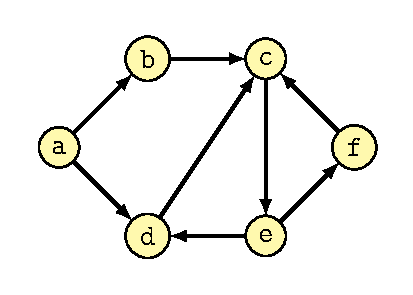
\includegraphics[width=0.70\textwidth,page=1]{scc.pdf}
\end{overprint}

\end{frame}

\begin{frame}{Componenti fortemente connesse}

\vspace{-6pt}
\begin{myboxtitle}[Domanda]
Quali sono le componenti fortemente connesse di questo grafo?
\end{myboxtitle}


\begin{overprint}
\onslide<1|handout:1>\centering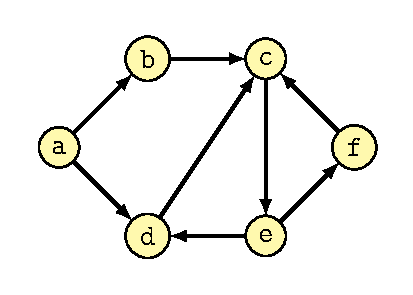
\includegraphics[width=0.70\textwidth,page=1]{scc.pdf}
\onslide<2|handout:2>\centering\includegraphics[width=0.70\textwidth,page=2]{scc.pdf}
\end{overprint}

\end{frame}

\begin{frame}{Soluzione "ingenua" (e non corretta)}

\BIL
\item Si applica l'algoritmo $\textsf{cc}()$ al grafo 
\item Purtroppo, il risultato dipende dal nodo di partenza
\EIL

\begin{overprint}
\onslide<1|handout:1>\centering\includegraphics[width=0.70\textwidth,page=3]{scc.pdf}
\onslide<2|handout:2>\centering\includegraphics[width=0.70\textwidth,page=4]{scc.pdf}
\onslide<3|handout:3>\centering\includegraphics[width=0.70\textwidth,page=5]{scc.pdf}
\end{overprint}

\end{frame}

\begin{frame}{Algoritmo di Kosaraju}

\vspace{-6pt}
\begin{myboxtitle}[Kosaraju Algorithm (1978)]
\BI
\item Effettua una visita DFS del grafo $G$
\item Calcola il grafo trasposto $G_t$
\item Esegui una visita DFS sul grafo $G_t$ utilizzando $\textsf{cc}$, esaminando i nodi nell'ordine inverso di tempo di fine della prima visita
\item Le componenti connesse (e i relativi alberi DF) rappresentano le componenti fortemente connesse di $G$
\EI
\end{myboxtitle}

\begin{Procedure}
\caption[A]{$\INTEGER[\,]$ \scc($\Graph\ G$)}

  $\Stack\ S = \topsort(G)$\REMR{First visit}
  $G^T = \textsf{transpose}(G)$\REMR{Graph transposal}
  $\Return\ \connectedcomponents(G^T, S)$\REMR{Second visit}

\end{Procedure}
\end{frame}

\begin{frame}{Ordinamento topologico su grafi generali}

\vspace{-6pt}
\begin{myboxtitle}[Idea generale]
Applicando l'algoritmo di ordinamento topologico su un grafo generale, siamo
sicuri che:
\BIL
\item se un arco $(u,v)$ non appartiene ad un ciclo, allora $u$ viene listato
prima di $v$ nella sequenza ordinata
\item gli archi di un ciclo vengono listati in qualche ordine, ininfluente
\EIL
\end{myboxtitle}


\BB{Utilizziamo quindi \texttt{topsort()} per ottenere i nodi in ordine decrescente di tempo di fine}

\end{frame}

\begin{frame}{Esecuzione 1: Ordinamento topologico}
    
\centering
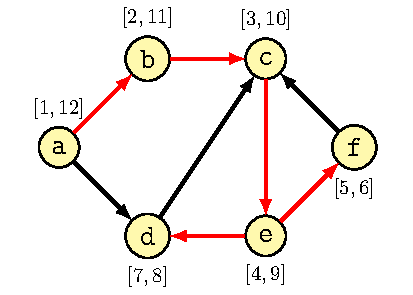
\includegraphics[width=0.7\textwidth, page=1]{scc3.pdf}

\Large
\texttt{Stack = \{ a, b, c, e, d, f \} }


\end{frame}

\begin{frame}{Calcolo del grafo trasposto}

\vspace{-6pt}
\begin{myboxtitle}[Grafo trasposto (Transpose graph)]
Dato un grafo orientato $G=(V,E)$, il \alert{grafo trasposto} $G_t = (V, E_T)$ ha gli stessi nodi e gli archi orientati in senso opposto.:
\[
E_T = \{ (u,v) ~|~ (v,u) \in E \}
\]
\end{myboxtitle}

\vspace{-9pt}
\begin{columns}[T]
\column{0.45\textwidth}
\begin{Procedure}
\caption[A]{$\INTEGER[\,]$ \textsf{transpose}($\Graph\ G$)}
  $\Graph\ G^T = \graphconstructor()$\;
  \lForEach{$u \in G.\VV()$}{ $G^T.\nodeins(u)$}
  \ForEach{$u \in G.\VV()$}{ 
    \ForEach{$v \in G.\adj(u)$}
    {
      $G^T.\edgeins(v,u)$\;
    }
  }
  \Return $G^T$\;
\end{Procedure}
\column{0.52\textwidth}
\BB{Costo computazionale: $O(m+n)$}
\BIL
\item $O(n)$ nodi aggiunti
\item $O(m)$ archi aggiunti
\item Ogni operazione costa $O(1)$
\EIL

\end{columns}

\end{frame}

\begin{frame}{Esecuzione 1: Grafo trasposto}
    
\begin{overprint}
\onslide<1|handout:0>\centering\includegraphics[width=0.7\textwidth,page=2]{scc3.pdf}
\onslide<2|handout:1>\centering\includegraphics[width=0.7\textwidth,page=3]{scc3.pdf}
\end{overprint}

\end{frame}


\begin{frame}[fragile]{Calcolo delle componenti connesse}
 
Invece di esaminare i nodi in ordine arbitrario, questa versione di
\texttt{cc()} li esamina nell'ordine LIFO memorizzato nello stack.

\vspace{-12pt}
\begin{columns}[T]
\column{0.45\textwidth}
\begin{Procedure}
\caption[A]{\connectedcomponents(\Graph $G$, \alert{$\Stack\ S$})}
$\INTEGER[\,]\ \components = \NEW\ \INTEGER[1 \mldots G.\textsf{size}()]$\;
\ForEach{$u \in G.\VV()$}
{
  $\components[u] = 0$
}
\INTEGER\ $\mathit{counter} = 0$\;
\While{\alert{\NOT\ $S.\textsf{isEmpty}()$}}
{
  \alert{$u = S.\textsf{pop}()$}\;
  \If{$\components[u] \Eq 0$}
  {
    $\mathit{counter} = \mathit{counter}+1$\;
    $\ccdfs(G, \mathit{counter}, u, \components)$\;
  }
}
\Return $\components$\;
\end{Procedure}
\column{0.51\textwidth}
\begin{Procedure}
\caption[A]{\ccdfs(\Graph $G$, \INTEGER\ $\mathit{counter}$, \Node\ $u$, $\INTEGER[\,]\ \components$)}
$\components[u] = \mathit{counter}$\;
\ForEach{$v \in G.\adj(u)$}
{
  \If{$\components[v] \Eq 0$}{$\ccdfs(G, \mathit{counter}, v, \components)$\;}
}
\end{Procedure}
\end{columns}
\end{frame}

\begin{frame}{Esecuzione 1: Componenti connesse}
    

\begin{overprint}
\onslide<1|handout:1>\centering\includegraphics[width=0.7\textwidth,page=4]{scc3.pdf}
\end{overprint}
\Large
\texttt{Stack = \{ a, b, c, e, d, f \} }

\end{frame}



\begin{frame}{SCC: The algorithm}
\vspace{-12pt}
\begin{Procedure}
\caption[A]{$\INTEGER[\,]$ \scc($\Graph\ G$)}

  $\Stack\ S = \topsort(G)$\REMR{First visit}
  $G^T = \textsf{transpose}(G)$\REMR{Graph transposal}
  $\Return\ \connectedcomponents(G^T, S)$\REMR{Second visit}

\end{Procedure}

\BB{Costo computazionale: $O(m+n)$}
\BIL
\item Ogni fase richiede $O(m+n)$
\EIL

\end{frame}

\begin{frame}{Esecuzione 2: Ordinamento topologico}

\centering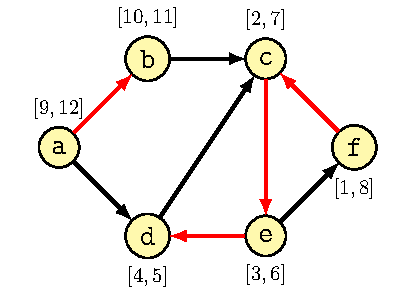
\includegraphics[width=0.7\textwidth,page=1]{scc4.pdf}

\Large
\texttt{Stack = \{ a, b, f, c, e, d \} }
\end{frame}

\begin{frame}{Esecuzione 2: Grafo trasposto}

% \begin{overprint}
% \onslide<1|handout:0>\centering\includegraphics[width=0.7\textwidth,page=2]{scc4.pdf}
%\onslide<2|handout:1>
\centering\includegraphics[width=0.7\textwidth,page=3]{scc4.pdf}
% \end{overprint}


\end{frame}

\begin{frame}{Esecuzione 2: Componenti connesse}

\centering\includegraphics[width=0.7\textwidth,page=4]{scc4.pdf}

\Large
\texttt{Stack = \{ a, b, f, c, e, d \} }

\end{frame}



\begin{frame}{Dimostrazione di correttezza}

\vspace{-6pt}
\begin{myboxtitle}[Grafo delle componenti]
$C(G) = (V_c, E_c)$
\BI
\item $V_c = \{ C_1, C_2, \ldots , C_k \}$, dove $C_i$ è la $i$-esima SCC of $G$
\item $E_c = \{ (C_i, C_j) | \exists (u_i, v_i) \in E: u_i \in C_i \wedge u_j \in C_j \}$
\EI
\end{myboxtitle}

\centering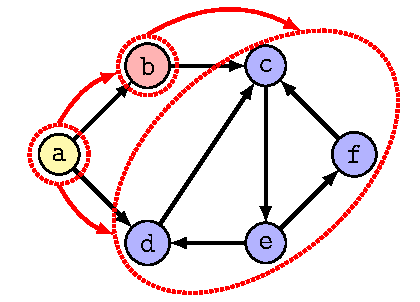
\includegraphics[width=0.5\textwidth,page=1]{scc2.pdf}
\end{frame}

\begin{frame}{Dimostrazione di correttezza}

\TwoCols{
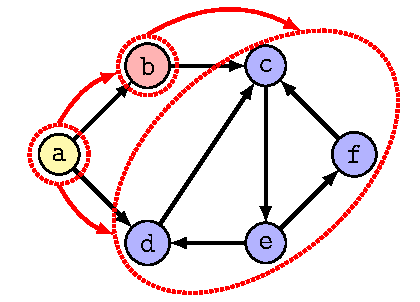
\includegraphics[width=0.8\textwidth,page=1]{scc2.pdf}
}{
\includegraphics[width=0.8\textwidth,page=6]{scc2.pdf}
}
\TwoColsCustom{0.73}{0.25}{
\BB{Qual è la relazione fra il grafo delle componenti di $G$ e il grafo delle componenti di $G_T$?}
\BB{Il grafo delle componenti è aciclico?}
}{

\vspace{20pt}
\pause $\alert{C(G^T) = [C(G)]^T}$

\vspace{28pt}
\pause \alert{SI}
}

\end{frame}


\begin{frame}{Dimostrazione di correttezza}

\vspace{-6pt}
\begin{myboxtitle}[Discovery time e finish time del grafo delle componenti]
\begin{align*}
	\ddt(C) &= \min \{ \ddt(u) | u \in C \} \\
	\dft(C) &= \max \{ \dft(u) | u \in C \}
\end{align*}
\end{myboxtitle}

\BB{Questi discovery/finish time corrispondono a i discovery/finish time del primo nodo visitato in $C$
}

\end{frame}

\begin{frame}{Dimostrazione di correttezza}

\vspace{-6pt}
\begin{myboxtitle}[Teorema]
Siano $C$ e $C'$ due distinte SCCs nel grafo orientato $G=(V,E)$. \\ 
Se c'è un arco $(C,C') \in E_c$, allora $\dft(C) > \dft(C')$.
\end{myboxtitle}

\TwoCols{
\includegraphics[width=1.0\textwidth,page=3]{scc2.pdf}
}{
\includegraphics[width=1.0\textwidth,page=4]{scc2.pdf}
}
\end{frame}

\begin{frame}{Dimostrazione di correttezza}

\vspace{-6pt}
\begin{myboxtitle}[Corollario]
Siano $C_u$ e $C_v$ due SCC distinte nel grafo orientato $G=(V,E)$. \\ 
Se c'è un arco $(u,v) \in E_t$ tale che $u \in C_u$ e $v \in C_v$, 
allora $\dft(C_u) < \dft(C_v)$.
\end{myboxtitle}

\TwoCols{
\begin{overprint}
\onslide<1|handout:1>
\begin{align*}
(u,v) \in E_t & \Rightarrow \\
(v,u) \in E & \Rightarrow \\
(C_v,c_u) \in E_c & \Rightarrow \\
\dft(C_v) > \dft(C_u) & \Rightarrow \\
\dft(C_u) < \dft(C_v) &
\end{align*}
\onslide<2|handout:2>
\begin{align*}
(b,a) \in E_t & \Rightarrow \\
(a,b) \in E & \Rightarrow \\
(C_a,C_b) \in E_c & \Rightarrow \\
12 = \dft(C_a) > \dft(C_b) = 11 & \Rightarrow \\
11 = \dft(C_b) < \dft(C_a) = 12 &
\end{align*}
\end{overprint}
}{
\includegraphics[width=1.0\textwidth,page=5]{scc2.pdf}
}
\end{frame}

\begin{frame}{Dimostrazione di correttezza}
    
\BIL
\item Se la componente $C_u$ e la componente $C_v$ sono connesse da un arco 
$(u,v) \in E_t$, allora:
\BI
\item Dal corollario, $\dft(C_u) < \dft(C_v)$
\item Dall'algoritmo, la visita di $C_v$ inizierà primma della visita di $C_u$
\EI
\item Non esistono cammini tra $C_v$ e $C_u$ in $G_t$
(altrimenti il grafo sarebbe ciclico)
\BI
\item Dall'algoritmo, la visita di $C_v$ non raggiungerà $C_u$,
\EI
\EIL

In altre parole, \texttt{cc()} assegnerà correttamente gli identificatori delle
componenti ai nodi.
\end{frame}    

\begin{frame}{Reality check}

\vspace{-6pt}
\begin{myboxtitle}[Algoritmo di Tarjan (1972)]
\BIL
\item Tarjan, R. E. "Depth-first search and linear graph algorithms", SIAM Journal on Computing 1(2): 146–160 (1972)
\item Algoritmo con costo $O(m+n)$ come Kosaraju
\item \EE preferito a Kosaraju in quanto necessita di una sola visita e non richiede il grafo trasposto
\EIL
\end{myboxtitle}

\begin{myboxtitle}[Applicazioni]
Gli algoritmi per SCC possono essere utilizzati per risolvere il problema
\alert{2-satisfiability} (\alert{2-SAT}), un problema di soddisfacibilità booleana con 
clausole composte da coppie di letterali.
\end{myboxtitle}

\end{frame}

\begin{frame}{Conclusioni}

\vspace{-6pt}
\IG{1.0}{graph-alg.pdf}    

\end{frame}

\end{document}
